\documentclass[9pt,twocolumn,twoside]{osajnl}

\journal{ao} % Choose journal (ao, aop, josaa, josab, ol)

% See template introduction for guidance on setting shortarticle option
\setboolean{shortarticle}{false}

\ifthenelse{\boolean{shortarticle}}{\colorlet{color2}{color2b}}{\colorlet{color2}{color2}} % Automatically switches colors for short articles

% Customized commands
\newcommand{\D}{\mathrm{d}}

\title{Camera response prediction for various capture settings using the spectral sensitivity and crosstalk model}

\author[1]{Author1}
\author[1,*]{Author2}
\affil[1]{State Key Laboratory of Modern Optical Instrumentation, College of Optical Science and Engineering, Zhejiang University, Hangzhou 310027, China}
\affil[*]{Corresponding author: xxx@zju.edu.cn}

\dates{Compiled \today}

\ociscodes{(040.1490) Camera; (150.1488) Calibration; (330.1710) Color, measurement; (330.1730) Colorimetry.}

\doi{\url{http://dx.doi.org/10.1364/ao.XX.XXXXXX}}

\begin{abstract}
	In this article, a camera response formation model is proposed to accurately predict the responses of images captured under various exposure settings. Differing from earlier works that estimated the camera relative spectral sensitivity, our model constructs the physical spectral sensitivity curves and device-dependent parameters that convert the absolute spectral radiances of target surfaces to the camera readout responses. With this model the camera responses to miscellaneous combinations of surfaces and illuminants could be accurately predicted, thus creating an ``imaging simulator'', by using which the colorimetric and photometric research based on the cameras would be much of convenience.
\end{abstract}

\setboolean{displaycopyright}{true}

\begin{document}
	
	\maketitle
	\thispagestyle{fancy}
	
	\ifthenelse{\boolean{shortarticle}}{\ifthenelse{\boolean{singlecolumn}}{\abscontentformatted}{\abscontent}}{}
	
	\section{Introduction}
	
	Determining the relationship between scene’s radiometric quantities and the camera responses is important for photographic calibrations and photometric measurements. Some applications, for instance, auto white balance and color correction in digital image processing pipeline, concern only about relative responses among channels. Some others, however, need to obtain the absolute responses of channels, e.g., using the camera as an irradiance or radiance detector.
	
	The camera response, i.e., pixel’s readout value, is mainly determined by the spectral radiance of the scene being imaged and the spectral sensitivity of the sensor. Specifically, for secondary reflection scene, the spectral radiance of a surface in the direction of optical axis is the function of the spectral intensity of light source, the spectral reflectance of the surface, and the geometrical relationship among three objects~\cite{Horn:79}. As the spectral sensitivity of the camera plays a significant role in image formation, considerable attention has been paid to it, which is also known as the spectral characterization.
	
	The traditional method to acquire the spectral sensitivity of an imaging device is to use a monochromator to generate near-monochromatic light in sequence spanning the visible range and simultaneously record the responses of the camera~\cite{Darrodi:15}. Though the monochromator method is easy-to-handle, it has two shortcomings. First, the measurement apparatus based on monochromators are expensive and require strictly controlled experimental environment, which is only possible in laboratories. Second, it does not take into account the crosstalk among adjacent pixels, which has been proved not to be ignorable in high-accuracy color reproduction~\cite{Getman:07}.
	
	To overcome the aforementioned shortcomings, researchers focused on estimating the camera spectral sensitivity by using imaging models and camera responses data, of which the prevailing methods can be grouped into two categories: algebraic method with constraints (abbreviated as AC henceforth) and basis function method (BF henceforth). The AC methods generally use Moore-Penrose pseudoinverse to find the solution that minimizes the cost function, being subject to some constraints, e.g., Tikhonov Regularization~\cite{Dyas:00}, Wiener filter~\cite{Urban:10} and first/second order derivatives~\cite{Barnard:02}, in order to satisfy conditions such as smoothness, unimodality and band-limitedness. The BF methods represent the camera spectral sensitivity curves with a linear combination of some basis functions, the choice of which varies for the different methods of this category~\cite{Finlayson:98,Zhao:09,Jiang:13}. A problem of BF methods, however, is that since the coefficients of the basis functions are obtained from a set of training samples, they might not suit to the testing sample whose spectral sensitivity has a rather distinct form.
	
	Most researches of the camera spectral sensitivity estimation go toward the goal that minimizes the difference between the estimated spectrum and the ground truth (usually measured by a monochromator). However, in most situations in color science and image technology, what really matters is how the spectral sensitivity influences the color rendering of imaging device. Considering that the camera spectral sensitivity is only a bridge that links the physical properties of real world, for example, surfaces' spectral radiances, to the digital output responses, the core of this study would be the prediction of the camera responses, rather than the spectral sensitivity. In addition, to our knowledge, the discussions about the spectral characterization have been limited to the acquisition of relative spectral sensitivity, but neglecting the physical mechanism that how a camera transforms the radiometric quantities into the corresponding digital quantities. In this study, we constructed a promisingly physical response formation model, illustrating the relationship between the absolute radiometric quantities, such as the spectral radiance (in $\text{W}\cdot\text{sr}^{-1}\cdot\text{m}^{-3}$), and the camera responses (raw format), given the capture settings of exposure time, aperture number, ISO sensitivity, and etc.
	
	\section{Methodology}\label{sec:methodology}
	
	\subsection{Response formation model}\label{sec:response formation model}
	
	The relative aperture, exposure time and ISO sensitivity are three main adjustable parameters that determine the camera raw responses before white balance and color correction. In this study, we took no account of relative aperture and kept it fixed, based on considerations of a) the change of the aperture would alter the optical property of the imaging system, for example, the angle between the optical axis and the light casting on the periphery of the sensor, being beyond the scope of this article, and b) for the lenses of most mobile devices the apertures are fixed, so a model excluding investigations of the aperture is acceptable.
	
	Leaving aside the influence to the noise level, the exposure time and ISO sensitivity are generally treated equivalently to the camera responses. That is, doubling ISO sensitivity but keeping exposure time unchanged has the same effect to the brightness of image as that doubling exposure time but keeping ISO sensitivity unchanged. However, this equivalence is somewhat untenable because of the inherent difference of the roles they play in the formation of the camera response: exposure time is the integral of the amount of photons arriving at the sensor, while ISO sensitivity is the digital amplification to an electric signal. Two experiments were carried out to support our points.
	
	A Nikon D3x DSLR camera, mounted with a Nikkor AF-S 24--120 $\text{f}/4$ ED VR zoom lens, was employed in our work. The lens was set to the focal length of 24mm and f-number of 4 throughout the works. The sensor in D3x consists of approximately 24M pixels, thus for every raw image we get a 6M-pixel RGB image before demosaicing. Unless otherwise specified, the word “pixel” in this article refers to a pixel having raw RGB triplet, and “the response of pixel” refers to that triplet.
	
	In the first experiment, we investigated how camera’s dark current level was impacted by different exposure time and ISO sensitivity settings. The dark current level of the camera is obtained by averaging $50\times50$ pixels in the central part of the image captured in dark room with a lens cap. As shown in Fig.~\ref{fig:1}(a), the rule that changing exposure time but with ISO sensitivity fixed has little or no impact on the dark current level holds for different ISO sensitivities (200 and 800). Then we captured dark-field images under different ISO sensitivities from 100 to 1600 in step of 1/3\,Ev, with exposure time unchanged. An obviously ascending trend for dark current level can be found in Fig.~\ref{fig:1}(b). It is worth stressing again that the spatially nonuniform noise (salt-and-pepper noise, etc.) was neglected by the average filter, only the uniform dark current level remained to be investigated.
	
	\begin{figure}[tbp]
		\centering
		\begin{minipage}{0.7\linewidth}
			\centering
			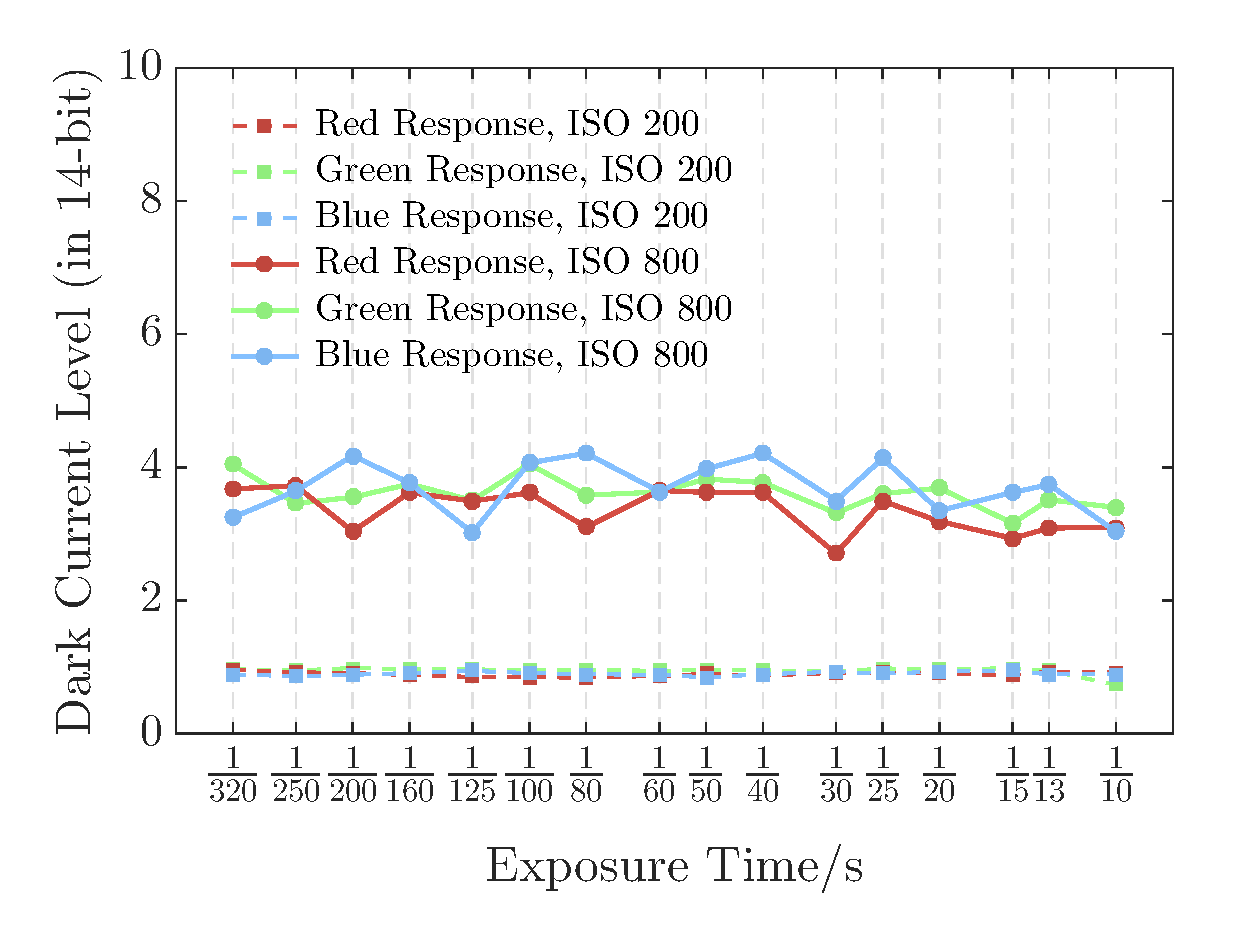
\includegraphics[width=\linewidth]{Fig1a}\\
			(a)
		\end{minipage}\\
		\vspace{0.5em}
		\begin{minipage}{0.7\linewidth}
			\centering
			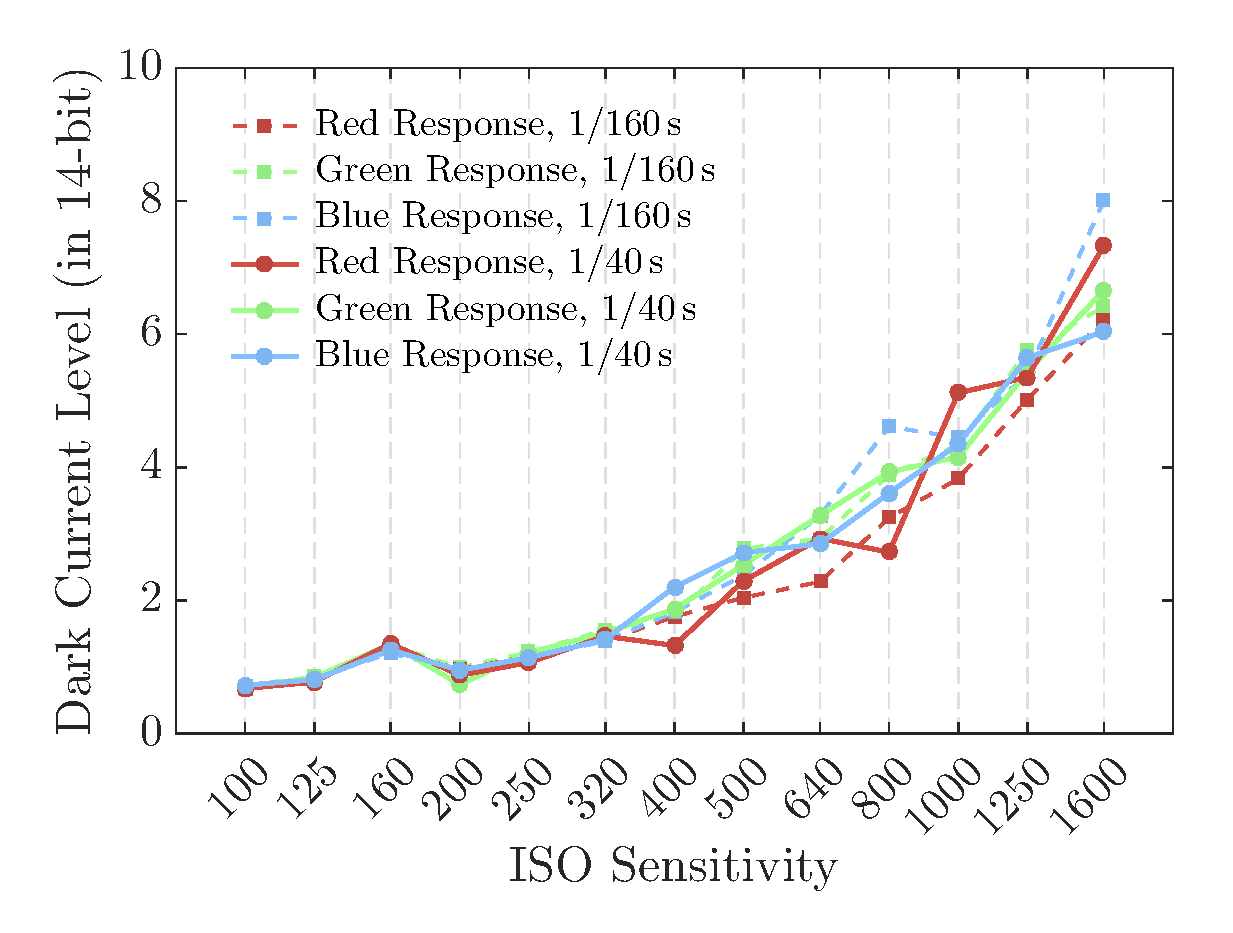
\includegraphics[width=\linewidth]{Fig1b}\\
			(b)
		\end{minipage}
	\caption{Dark current levels of Nikon D3x under (a) different exposure times and (b) different ISO sensitivities.}
	\label{fig:1}
\end{figure}

In the second experiment, we captured X-Rite ColorChecker Digital Semi-Gloss (DSG) with different combinations of exposure time and ISO sensitivity. The camera responses of 96 color patches under different settings were recorded, with 44 repeated neutral colors around the ColorChecker DSG excluded. The responses of one patch under different capture settings were normalized so that the response under the setting of ISO 100 and 1/15\,s exposure time was equal to 1, as shown in Fig.~\ref{fig:2}, in which, for clarity, only 48 randomly selected patches are plotted. The asterisk at the exposure time denotes that this response was adjusted in order to make the products of ISO and exposure time invariant. For example, the response under ISO 800 and 1/125\,s was multiplied by 125/120 to get the anticipated response under ISO 800 and 1/120\,s, because the exposure time cannot be manually set to 1/120\,s for D3x (This conversion is valid only when the camera responses are linear with respect to exposure time, which can be demonstrated by Fig.~\ref{fig:3}.). The inclines of lines illustrate the nonequivalence between exposure time and ISO sensitivity. Consequently, if the traditional spectral characterization methods were adopted to predict the camera responses under different capture settings, errors would be inevitable.

\begin{figure}[tbp]
	\centering
	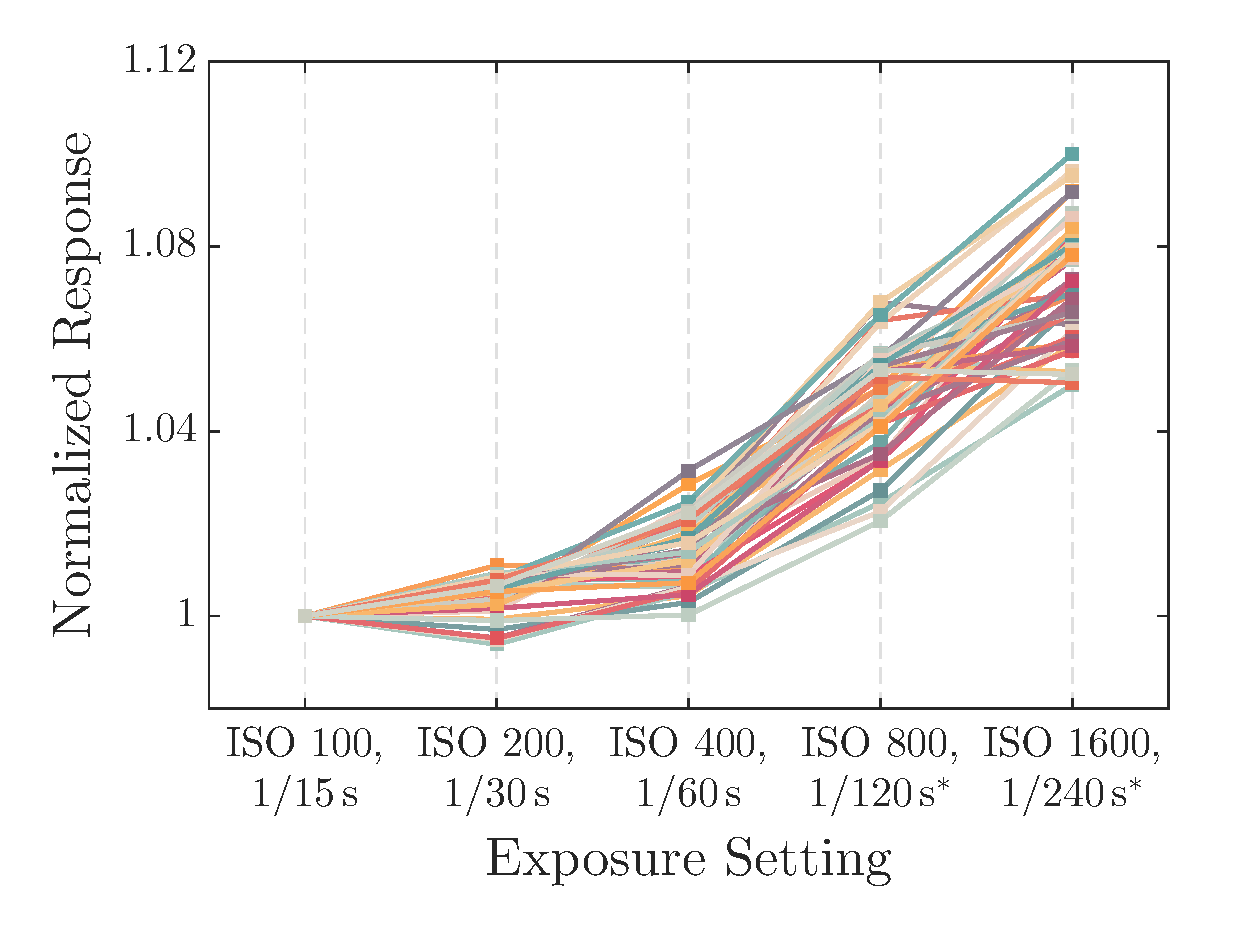
\includegraphics[width=.75\linewidth]{Fig2}
	\caption{The green channel’s normalized responses of color samples under different combinations of exposure time and ISO sensitivity.}
	\label{fig:2}
\end{figure}

Based on the above two experiments, the camera response of the pixel at position $\mathbf{x}$ can be expressed as
\begin{equation}
p(\mathbf{x}) = f_\text{S}\cdot\Big(\int_\tau Q(\mathbf{x})\,\D{t}+c_1\Big)+n\,,
\label{eq:1}
\end{equation}
where $f_\text{S}$ is a function of ISO sensitivity, $\tau$ represents exposure time, $Q(\textbf{x})$ is the amount of electrons converted from photons by the photosensitive sensor in unit time at pixel $\textbf{x}$, $n$ is the random noise with zero mean and finite variance, thus can be neglected by applying an average filter. The existence of small positive constant $c_1$ explains the nonequivalence of exposure time and ISO sensitivity. When no light enters into the camera, the response, i.e., the dark current level, is the sole function of ISO sensitivity. If the product of $f_\text{S}$ and $\tau$ is invariant, the shift of response has the same direction as the shift of ISO sensitivity.

According to the definition of $Q(\mathbf{x})$ in \eqref{eq:1}, it can be decomposed into two part:
\begin{equation}
Q(\mathbf{x}) = \int_\Omega{}E(\lambda,\mathbf{x})S_\text{Q}(\lambda)\,\D{\lambda}\,,
\label{eq:2}
\end{equation}
where $S_\text{Q}(\lambda)$ is the informally defined quantum efficiency in our research, in $\text{m}^2\cdot\text{W}^{-1}\cdot\text{s}^{-1}$ (because $\Phi$ is a dimensionless unit), i.e., the sensitivity of sensor converting the spectral irradiant to the amount of electrons. $E(\lambda,\mathbf{x})$ is the spectral irradiance, in $\text{W}\cdot\text{m}^{-3}$, on the pixel $\mathbf{x}$, $\Omega$ is the spectrum range of integral, usually the visible range because the UV and IR portions in $E(\lambda,\mathbf{x})$ have been cut off by the filters.

In this article, $\Phi(\mathbf{x}) = \int_\tau Q(\mathbf{x})\,\D{t}$ is considered as a ``physical term'', which is only contributed by the spectral irradiance on the sensor, the quantum efficiency and the integral time, in comparison with the ``digital terms'' $f_\text{S}$ and $c_1$, which are involved in the process of digital discrete sampling in the circuits. When the spectral irradiance and the quantum efficiency are time-invariant during one shoot, the physical term can be simplified as $\Phi(\mathbf{x})=\tau Q(\mathbf{x})$.

The nonlinearity between the irradiance on the sensor and the camera readout response has been discussed in literatures~\cite{Barnard:02,Fiorentin:05,Thomson:01}. In our model, the nonlinearity is assumed to be introduced during the digital signal processing, like electronic signal amplification, rather before the absorption of lights and the collection of charges.

If the nonlinearity is independent of the capture settings, \eqref{eq:1} becomes 
\begin{equation}
p(\mathbf{x}) = f_\text{S}\cdot\bigg[\Big(\int_\tau Q(\mathbf{x})\,\D{t}+c_1\Big)^\beta+c_2\bigg]\,,
\label{eq:3}
\end{equation}
where $c_1$, $c_2$ and $\beta$ are parameters determining the nonlinearity of responses, subjected to $c_1^{\,\beta}+c_2>0$. Fig.~\ref{fig:3} plots the scatter diagram of green channel's normalized responses with respect to exposure time for D3x (saturated responses have been removed), in which the responses are extracted from five neutral patches in the X-Rite ColorChecker Classic (the darkest one not included) and normalized according to their radiance.

\begin{figure}[tbp]
	\centering
	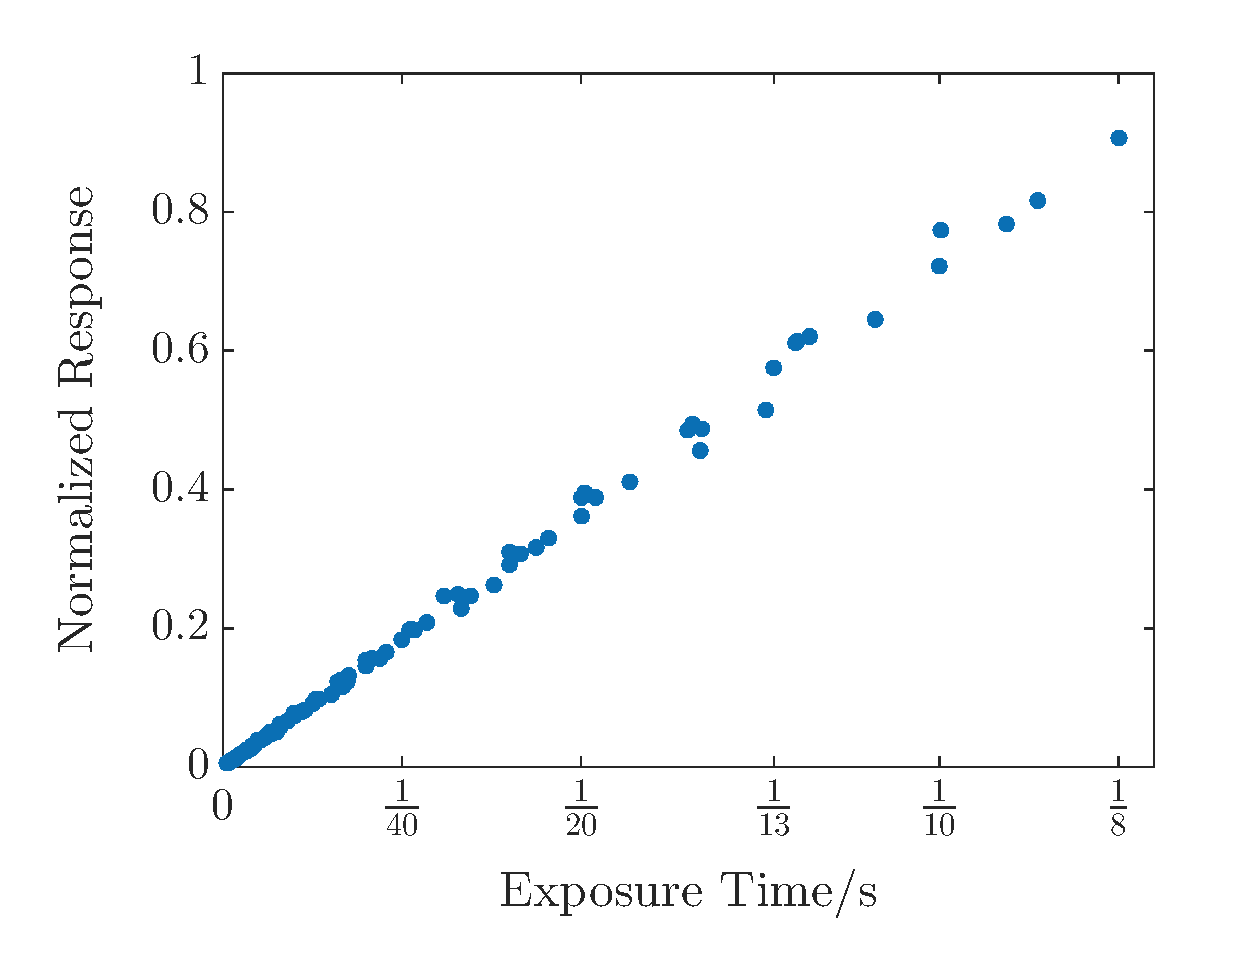
\includegraphics[width=.73\linewidth]{Fig3}
	\caption{The linearity of green channel for Nikon D3x with respect to exposure time}
	\label{fig:3}
\end{figure}

In a typical imaging system, the spectral irradiance on a pixel $\mathbf{x}$, $E(\lambda,\mathbf{x})$, is related to the scene’s spectral radiance $l(\lambda,\mathbf{x})$ (in $\text{W}\cdot\text{sr}^{-1}\cdot\text{m}^{-3}$) as follows~\cite{Horn:79}: 
\begin{equation}
E(\lambda,\mathbf{x}) = \frac{\pi}{4}l(\lambda,\mathbf{X})T(\lambda)\Big(\frac{d}{f_p}\Big)^2\cos^4\alpha\,,
\label{eq:4}
\end{equation}
where $\mathbf{X}$ represents the position in space corresponding to $\mathbf{x}$ by general projective camera model~\cite{Hartley:04}, $d$ is the diameter of aperture, $f_p$ is the focal length of optical system and the ratio of focal length to aperture diameter is known as relative aperture or f-number, $\alpha$ is the angle between the optical axis and the line linking $\mathbf{X}$ and $\mathbf{x}$. When the relative aperture is fixed, $g = \left.\pi\cos^4\alpha\middle/4F^2\right.$ is a geometric constant only depending on the position of the pixel $\mathbf{x}$. $T(\lambda)$ is the total transmission of the imaging system and can be decomposed as follows for Bayer pattern cameras:
\begin{equation}
T(\lambda) = T_\text{o}(\lambda)T_\text{c}^{(k)}(\lambda)\,,
\label{eq:5}
\end{equation}
where $T_\text{o}(\lambda)$ is the transmission of optical system (lens, low-pass filter, IR filters, etc.), $T_\text{c}^{(k)}(\lambda)$ is the transmission of color filter on $k=\text{R, G, B}$ channel.

Combining Eqs.~(\ref{eq:2}) and~(\ref{eq:4}), and considering that all spectra are invariant during one exposure, the physical term $\Phi$ of $k$ channel becomes:
\begin{equation}
\Phi^{(k)}(\mathbf{x}) = \tau Q(\mathbf{x}) = g\tau\int_\Omega{}l(\lambda,\mathbf{X})T_\text{o}(\lambda )T_\text{c}^{(k)}(\lambda)S_\text{Q}(\lambda)\,\D{\lambda}\,.
\label{eq:6}
\end{equation}

In \eqref{eq:6}, it is assumed that the spectral irradiance on pixel $\mathbf{x}$ derives \textit{only} from the light penetrating through the color filter over the pixel. Nevertheless, when the incident ray is oblique, the light between two adjacent pixels may not be completely isolated, as illustrated in Fig.~\ref{fig:4}, then the crosstalk effect arises.

\begin{figure}[tbp]
	\centering
	\includegraphics[width=.65\linewidth]{Fig4}
	\caption{The crosstalk effect on sensor between red and green pixels.}
	\label{fig:4}
\end{figure}

Considering an extreme but articulate example: given a sensor with RGB Bayer filter stamped, the red filter of which is only sensitive to the energy within the wavelength range of 550--700nm and the green counterpart is within 450--600nm. The amplitude of the spectral sensitivity curve of the red channel at 650nm can be calculated when capturing a scene illuminated by near-monochromatic light of 650nm central wavelength. Apparently the green channel has no response because 650nm light is filtered out by the green filter. Now the near-monochromatic light source is replaced by a hypothetical source whose spectrum consists of two narrow peaks locating at 500nm and 650nm, respectively. If there exists crosstalk between the adjacent red and green pixel, in other words, part of light penetrating through the green filter arrives at the pixel beneath the red filter, then the response of that red pixel is impacted by both 650nm and 500nm light, thus differing from the value measured by a monochromator. This example explains why the camera responses reconstructed using the spectral sensitivity measured by a monochromator will deviate from the actual values, especially for the cameras on mobile devices that have stronger channels crosstalk due to the low-end lenses and poor-assembled micro-lens arrays.

It is suggested that the crosstalk in Bayer filter sensor only occurs between the adjacent pixels~\cite{Getman:07}, thus for an RGGB pattern sensor, the physical term of three channels can be derived as
\begin{equation}
\left\{\begin{aligned}
\Phi^\text{R} &= g\tau\int_\Omega{}l\,T_\text{o}\left[C_\text{RR}T_\text{c}^\text{R}+C_\text{GR}T_\text{c}^\text{G}\right]S_\text{Q}\,\D{\lambda} \\
\Phi^\text{G} &= g\tau\int_\Omega{}l\,T_\text{o}\left[C_\text{RG}T_\text{c}^\text{R}+C_\text{GG}T_\text{c}^\text{G}+C_\text{BG}T_\text{c}^\text{B}\right]S_\text{Q}\,\D{\lambda} \\
\Phi^\text{B} &= g\tau\int_\Omega{}l\,T_\text{o}\left[C_\text{GB}T_\text{c}^\text{G}+C_\text{BB}T_\text{c}^\text{B}\right]S_\text{Q}\,\D{\lambda}
\end{aligned}\right.\,,
\label{eq:7}
\end{equation}
where the coefficient $c_{kk'}$ weights the intensity of the crosstalk coefficient from pixel $k$ to $k'$. Since red pixels and blue pixels always locate diagonally, $c_\text{RB} = c_\text{BR}\equiv0$.

The integral in \eqref{eq:7} can be converted to the summation and rewritten in the matrix form as
\begin{equation}
\mathbf{\Phi} = g\tau(\Delta\lambda)\mathbf{C}\cdot\mathbf{S}^\intercal\cdot\mathbf{l}\,,
\label{eq:8}
\end{equation}
where $\Phi = \left[\Phi^\text{R},\Phi^\text{G},\Phi^\text{B}\right]^\intercal$ is the physical terms triplet, $\mathbf{l}$ is a vector representing the spectral radiance on $\mathbf{X}$, $\mathbf{S} = \left[\mathbf{S}^\text{R},\mathbf{S}^\text{G},\mathbf{S}^\text{B}\right]^\intercal$ and $\mathbf{S}^{(k)} = \mathbf{T}_\text{o}\mathbf{T}_\text{c}^{(k)}\mathbf{S}_\text{Q}$ are the element-wise products of the spectral transmissions and quantum efficiency, thereby called the camera spectral sensitivity of $k$ channel in this article. $\Delta\lambda$ is the wavelength interval, in accordance with the sampling interval of $l(\lambda)$. The crosstalk matrix $\mathbf{C}$ consists of 7 coefficients:
\begin{equation}
\mathbf{C} = \begin{bmatrix}
C_\text{RR} & C_\text{GR} & 0 \\
C_\text{RG} & C_\text{GG} & C_\text{BG} \\
0			& C_\text{GB} & C_\text{BB} \\
\end{bmatrix}\,.
\label{eq:9}
\end{equation}

Given the uniform spectral radiance on a small region around the point $\mathbf{X}$, we can predict its camera response by Eqs.~(\ref{eq:8}) and~(\ref{eq:3}) as
\begin{equation}
\hat{\mathbf{p}} = f_\text{S}\cdot\bigg\{\Big[g\cdot{}\tau \cdot\Delta\lambda\cdot\mathbf{C}\cdot\mathbf{S}^\intercal\cdot\mathbf{l} + c_1\Big]^\beta + c_2\bigg\}\,.
\label{eq:10}
\end{equation}

\eqref{eq:10} is the general form of the camera response formation model in this study.

\subsection{Spectral sensitivity and parameters estimation}\label{sec:estimation}

The camera spectral sensitivity, the crosstalk coefficients and the nonlinear parameters can be estimated by minimizing the errors between the predicted responses $\hat{\mathbf{p}}$ and the actually recorded responses $\mathbf{p}$ under different capture settings.

\subsubsection{Optimization method}\label{sec:optimization method}

Most previous literatures used relative errors in camera RGB space as the cost function to be minimized~\cite{Urban:10,Barnard:02,Finlayson:98,Huynh:14,Ebner:07,Prasad:13}, because of its operational convenience. However, it’s more appropriate to evaluate the errors in a perceptually uniform color space rather than a device-dependent color space, based on the considerations of a) our goal is to predict camera responses as perceptively accurate as possible, whereas in the camera RGB space, the smallest relative error cannot guarantee the best visual conformity, and b) the device-dependent responses are meaningless for photographic calibrations or photometric measurements.

The standard formula of CIEDE2000 ($\Delta{}E_{00}$) was adopted to measure the color differences between the predicted responses and the actual camera responses. Before the parameters estimation, the colorimetric characterization was performed to convert the camera RGBs in device-dependent color space to CIE colorimetric parameters like CIE1931 XYZ in device-independent color space. Since capturing settings were variant in our experiment, the traditional polynomial color correction (PCC) approach was unsuitable, otherwise it would cause a significant problem when the data were scaled by the changes of scene radiance or exposure. As suggested by~\cite{Finlayson:15}, the root-polynomial color correction (RPCC) regression was utilized to perform the colorimetric characterization.

For a high accuracy, the root-polynomial expansions of 4\textsuperscript{th} degree are used:
\begin{equation}
\begin{split}
\bar{\boldsymbol{\rho}}_{4,3} = \biggl(& r, g, b, \sqrt{rg}, \sqrt{gb}, \sqrt{rb},\biggr. \\
& \sqrt[3]{rg^2}, \sqrt[3]{gb^2}, \sqrt[3]{rb^2}, \sqrt[3]{gr^2}, \sqrt[3]{bg^2}, \sqrt[3]{br^2}, \sqrt[3]{rgb}, \\
& \sqrt[4]{rg^3}, \sqrt[4]{gb^3}, \sqrt[4]{rb^3}, \sqrt[4]{gr^3}, \sqrt[4]{bg^3}, \sqrt[4]{br^3}, \\
& \biggl.\sqrt[4]{r^2gb}, \sqrt[4]{g^2rb}, \sqrt[4]{b^2rg}\biggr)^\intercal\,.
\end{split}
\label{eq:11}
\end{equation}

A $3\times22$ color space conversion matrix $\mathbf{M}$ can be calculated using the nonlinear least squares method such that the summing $\Delta{}E_{00}$ between the measured tristimulus values $\mathbf{q}_i$ and the converted values $\hat{\mathbf{q}}_i = \mathbf{M}\boldsymbol{\rho}_i$ is minimized.

The responses of 96 color samples, captured under the setting of 1/15\,s exposure time and ISO 100, were utilized as training data to perform RPCC of 4\textsuperscript{th} degree expansions and calculate $\mathbf{M}$. The responses obtained under other capture settings were employed as testing data to test the performance of colorimetric characterization. Fig.~\ref{fig:5} illustrates the CIEDE2000 color differences between the measured and converted tristimulus values for different capture settings, in which the error bars represent the 95\% confidence interval of 96 samples under one capture setting.

\begin{figure}[tbp]
	\centering
	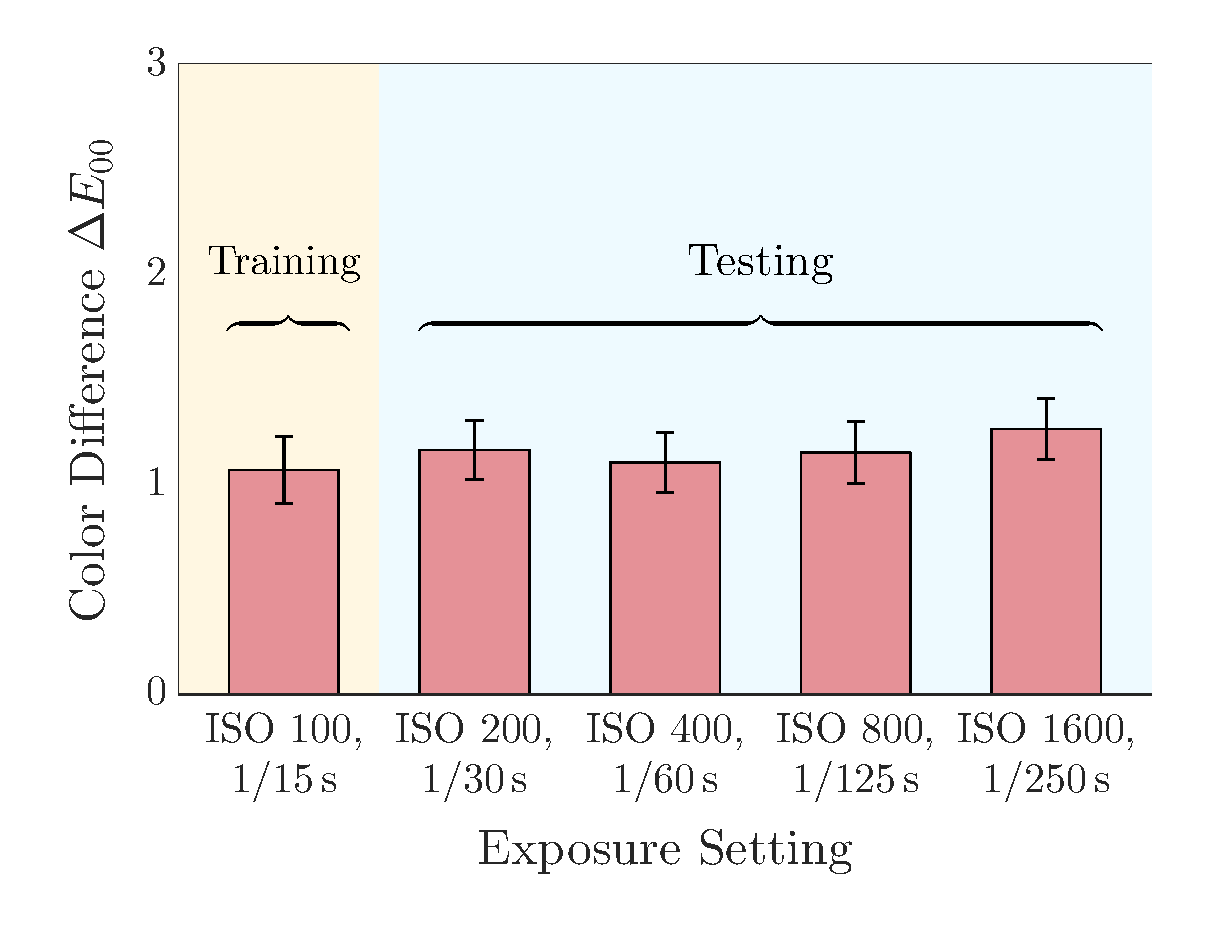
\includegraphics[width=.75\linewidth]{Fig5}
	\caption{CIEDE2000 color differences of colorimetric characterization under different exposure settings, using PRCC regression with 4\textsuperscript{th} degree expansions.}
	\label{fig:5}
\end{figure}

Although the colorimetric characterization may introduce some additional errors, it applies equally to the actual and the predicted camera RGBs. The cost function in our experiment thus becomes the color difference $\Delta{}E_{00}$ between $\mathbf{M}\boldsymbol{\rho}$ and $\mathbf{M}\bar{\boldsymbol{\rho}}$, where $\boldsymbol{\rho}$ and $\bar{\boldsymbol{\rho}}$ are expanded form of $\mathbf{p}$ and $\bar{\mathbf{p}}$ respectively.

Now, the problem can be summarized as to find the camera spectral sensitivities of three channels, the crosstalk coefficients and the nonlinear parameters in \eqref{eq:10} to minimize the cost function of
\begin{equation}
\mathcal{F} = \frac{\sum\limits_{i = 1}^N\Delta{}E_{00}\left(\mathbf{M}\boldsymbol{\rho}_i, \mathbf{M}\hat{\boldsymbol{\rho}}_i\right)}{N} + \mu\max\big\{\Delta{}E_{00}\left(\mathbf{M}\boldsymbol{\rho}_i, \mathbf{M}\hat{\boldsymbol{\rho}}_i\right)\big\}\,,
\label{eq:12}
\end{equation}
where $\mu$ is an adjustable factor that takes into account the maximum color difference in all samples to avoid too distinguishing errors. It was empirically set to 0.1 in our manipulation.

The interior-point method is selected as the algorithm to solve the constrained nonlinear optimization problem~\cite{Byrd:99,Forsgren:02}, since the response formation model \eqref{eq:10} is a power function and the gradient can hardly be provided during optimization. In Mathwork Matlab versions later than 2007, the interior-point method for constrained nonlinear optimization is alternative in \verb|fmincon| function.

\subsubsection{Operational details}\label{sec:operational details}

Similar to other nonlinear optimization algorithms, the interior-point method requires the initial guess to start the minimum search. The initial estimation of the camera spectral sensitivity is obtained analogous to~\cite{Barnard:02}, but with the L-curve method to find the suitable regularization parameter.

The training data are the spectral radiances (in $\text{W}\cdot\text{sr}^{-2}\cdot\text{m}^{-3}$) of $N$ color samples in ColorChecker DSG, measured by Konica Minolta CS-2000 spectroradiometer, as well as the corresponding camera responses under different capture settings. Let m denote the number of capture settings adopted, the camera responses of N samples under different settings can then be rearranged as an $mN\times3$ matrix:
\begin{equation}
\mathbf{r} = \left[\mathbf{r}_1;\ldots;\mathbf{r}_m\right]\,,
\label{eq:13}
\end{equation}
where $\mathbf{r}_i$ is the responses combination of $N$ samples under the $i\textsuperscript{th}$ capture setting:
\begin{equation}
\mathbf{r}_i = \left[\mathbf{p}_1^\intercal;\ldots;\mathbf{p}_N^\intercal\right]_{i-\text{setting}}\,.
\label{eq:14}
\end{equation}

The spectral radiances corresponding to $N$ samples can also be rearranged as a $mN\times{}M$ matrix $\mathbf{L}$, where $M$ is the number of wavelengths defined by the spectroradiometer. When the lighting condition and samples’ reflectance attributes can be seen as constant during $m$ shoots, the spectral radiances of $N$ samples can be duplicated $m$ times rather than performing $mN$ measurements:
\begin{equation}
\mathbf{L} = {\large[}\underbrace{\mathcal{L};\ldots;\mathcal{L}}_m{\large]}\,,
\label{eq:15}
\end{equation}
where $\mathcal{L}$ is the combination of the spectral radiance data of $N$ samples:
\begin{equation}
\mathcal{L} = \left[\mathbf{l}_1^\intercal;\ldots;\mathbf{l}_N^\intercal\right]\,,
\label{eq:16}
\end{equation}
and $\mathbf{l}_j$ is the spectral radiance vector of $j\textsuperscript{th}$ color sample containing $M$ elements.

In the initial guess phase, the crosstalk and nonlinearity in the response formation model is neglected, so \eqref{eq:10} can be simplified as
\begin{equation}
\mathbf{\hat{p}}_0 = c\mathbf{S}^\intercal\cdot\mathbf{l}\,,
\label{eq:17}
\end{equation}
where $c = f_\text{S}\,gt(\Delta\lambda)$ is a scalar determined by the capture setting. For convenience, the exposure time $T$ is measured in seconds and $f_\text{S}$ is obtained by dividing ISO value recorded in the image header by 100.

According to \eqref{eq:17}, the response formation model for all training color samples in initial guess phase has the matrix form:
\begin{equation}
\mathbf{r} = \text{diag}(\mathbf{s})\cdot\mathbf{L}\cdot\mathbf{S}\,,
\label{eq:18}
\end{equation}
where $\mathbf{s} = \left[s_1;\ldots;s_{mN}\right]$ is a vector containing different $c$ for corresponding captures.

Solving $\mathbf{S}$ directly using Moore–Penrose pseudoinverse or SVD would get an unstable solution, since it is an ill-posed problem, in which a small perturbation during measurement would cause a large deviation from the exact solution\cite{Forsgren:02}. Therefore, an $(M-2)\times{}N$ discrete approximation of the second derivative operator $\mathcal{R}$ is applied as the regularization constraint:
\begin{equation}
\mathcal{R} = \begin{bmatrix}
-1	& 2  & -1 	 &  	  &  	   &  	\\
& -1 & 2 	 & -1 	  &  	   &  	\\
&	 & \ddots& \ddots & \ddots &  	\\
&	 & 	 	 & -1 	  & 2 	   & -1 \\
\end{bmatrix}\,,
\label{eq:19}
\end{equation}
so that the least-square problem for $k\textsuperscript{th}$ channel that minimize the relative error becomes
\begin{equation}
\left[
\begin{array}{c}
\mathbf{L}_\text{rel}^{(k)}\\\hline
\lambda\mathcal{R}
\end{array}
\right]%
\mathbf{S}^{(k)} =%
\left[
\begin{array}{c}
\mathbf{1}\\\hline
\mathbf{0}
\end{array}
\right]\,,
\label{eq:20}
\end{equation}
where $\mathbf{L}_\text{rel}^{(k)} = \text{diag}(\mathbf{s})\cdot\Big[\text{diag}\big(\mathbf{r}^{(k)}\big)\Big]^{-1}\cdot\mathbf{L}$.

Regularization parameter $\lambda$ is the only factor that modulates the smoothness of the camera spectral sensitivity $\mathbf{S}^{(k)}$. The smaller $\lambda$ is, the smaller residual error, i.e.\ $\big\|\left.\left[\text{diag}(\mathbf{c})\cdot\mathbf{L}\cdot\mathbf{S} - \mathbf{r}\right]\middle/\mathbf{r}\right.\big\|_2$, we could get, but large oscillation may occur to the solution curve and deviates it from exact shape. Conversely, the greater $\lambda$ is, the smaller regularization error, i.e.\ $\big\|\lambda\mathcal{R}\mathbf{S}\big\|_2$, we could achieve, thus ensuring the smoothness of $\mathbf{S}^{(k)}$ at the expense of greater residual error.

The L-curve is a convenient graphical tool for analysis of discrete ill-posed problems, which is a log-log scale plot of the (semi)norm of the regularized solution versus the corresponding residual norm. An essential feature of the L-curve is that this optimal regularization parameter is not far from the regularization parameter that corresponds to the L-curve’s corner. In other words, by locating the corner of the L-curve one can compute an approximation to the optimal regularization parameter and thus, in turn, compute a regularized solution with a good balance between the two error types~\cite{Hansen:94}.

In this case, we combine the responses from three channels together to compute a global optimal regularization parameter $\lambda_0$, which can be applied to \eqref{eq:20} consistently for three channels.

First, the compact generalized singular value decomposition (CGSVD) was performed to the matrix pair $\left(\mathbf{L}'_\text{rel}, \mathcal{R}'\right)$ in the form of
\begin{equation}
\mathbf{L}'_\text{rel} = \mathbf{U}%
\begin{bmatrix}
\mathbf{\Sigma} & \mathbf{0} \\
\mathbf{0}		& \mathbf{I}
\end{bmatrix}%
\mathbf{X}^{-1}\,,\quad%
\mathcal{R}' = \mathbf{V}%
\begin{bmatrix}
\mathbf{M} & \mathbf{0}
\end{bmatrix}%
\mathbf{X}^{-1}\,,
\label{eq:21}
\end{equation}
where $\mathbf{L}'_\text{rel}$ and $\mathcal{R}'$ are block diagonal matrix constructed from $\mathbf{L}_\text{rel}^{(k)}$ and $\mathcal{R}$ respectively:
\begin{equation}
\mathbf{L}'_\text{rel} =%
\begin{bmatrix}
\mathbf{L}_\text{rel}^\text{R} & 								& \\
& \mathbf{L}_\text{rel}^\text{G} & \\
&								& \mathbf{L}_\text{rel}^\text{B}
\end{bmatrix}\,,\quad%
\mathcal{R}' =%
\begin{bmatrix}
\mathcal{R} &			  &	\\
& \mathcal{R} & \\
&			  & \mathcal{R}
\end{bmatrix}\,.
\label{eq:22}
\end{equation}

The columns of $\mathbf{U}$ and $\mathbf{V}$ are orthonormal, $\mathbf{X}$ is nonsingular, $\mathbf{\Sigma}$ and $\mathbf{M}$ are $3(M-2)\times3(M-2)$ diagonal matrices:
\begin{equation*}
\mathbf{\Sigma} = \text{diag}(\sigma_1,\ldots,\sigma_{3(M-2)})\,,\quad%
\mathbf{M} = \text{diag}(\mu_1,\ldots,\mu_{3(M-2)})\,.
\end{equation*}

The entries of $\mathbf{\Sigma}$ and $\mathbf{M}$ are non-negative and ordered such that $0\le\sigma_1\le\ldots\le\sigma_{3(M-2)}\le1$, $1\ge\mu_1\ge\ldots\ge\mu_{3(M-2)}>0$, and they are normalized such that $\sigma_i^2 + \mu_i^2 = 1$, for $i = 1,\ldots,3(M-2)$.

Then, by using $\mathbf{U}$, $\mathbf{\Sigma}$ and $\mathbf{M}$, the residual error versus regularized error, as a function of $\lambda$, can be plotted on a log-log coordinate, forming an L-shape curve. At the corner of L-curve the optimal regularization parameter $\lambda_0$ can be located, as demonstrated in Fig.~\ref{fig:6}. In this case, the responses from $N=48$ color samples under $m=5$ capture settings are used as training data, and $M=81$ wavelengths are sampled from the range of 380--780nm in an interval of 5nm.

\begin{figure}[tbp]
	\centering
	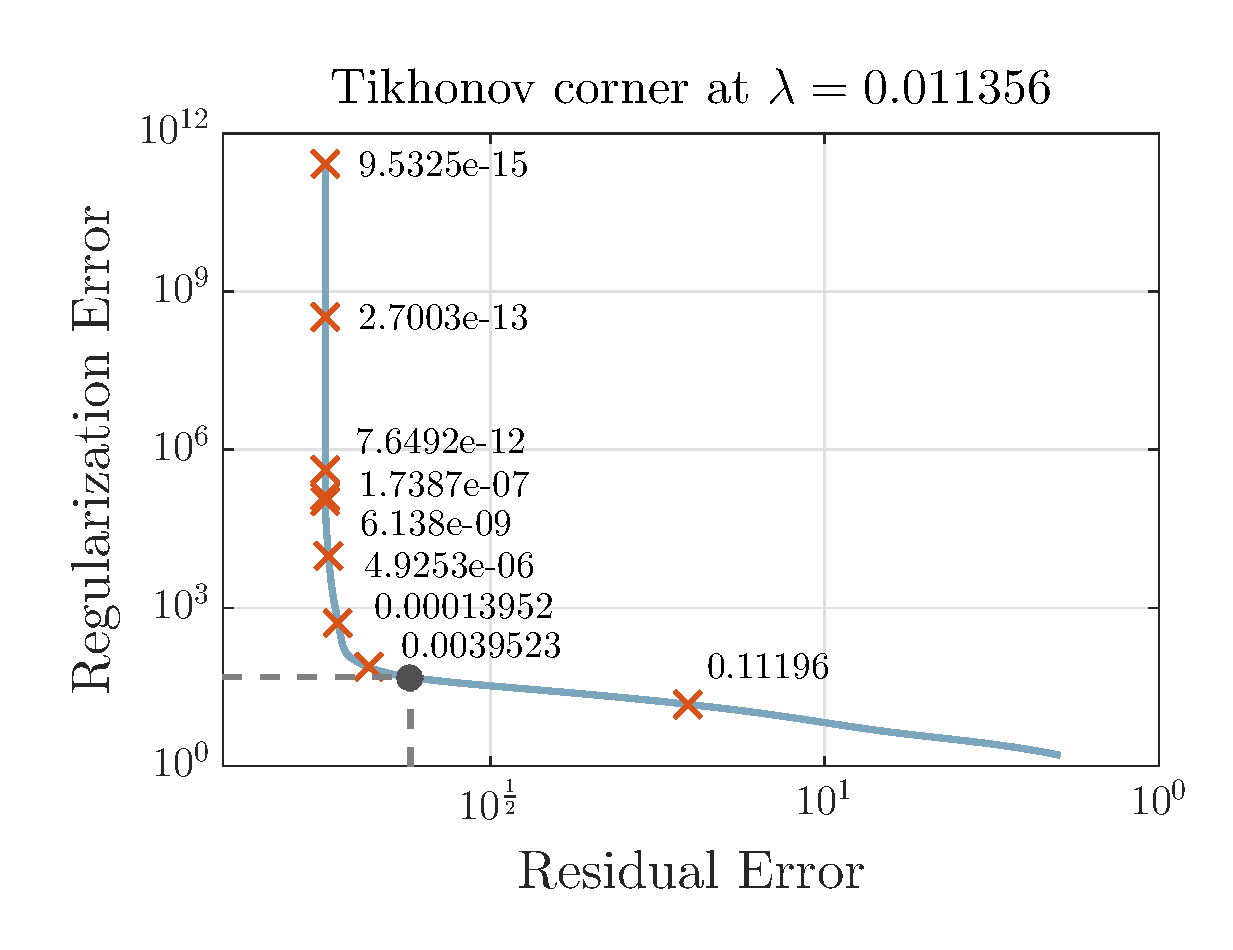
\includegraphics[width=.75\linewidth]{Fig6}
	\caption{The L-curve of the regularization. The circle denotes the corner of  L-curve, corresponding to the optimal regularization parameter $\lambda$.}
	\label{fig:6}
\end{figure}

The initial guess, $\mathbf{S}_0$, of $\mathbf{S}$ can be obtained by solving \eqref{eq:20} for three channels, respectively, using the nonnegative least squares method~\cite{Lawson:95} with the optimal global parameter $\lambda_0$ as regularization.

When the initial camera spectral sensitivity is known, a set of simplified estimated camera response $\hat{\mathbf{r}}_0$ can be constructed using \eqref{eq:18}:
\begin{equation}
\hat{\mathbf{r}}_0 = \text{diag}(\mathbf{s})\cdot\mathbf{L}\cdot\mathbf{S}_0\,.
\label{eq:23}
\end{equation}

Next, the initial values of nonlinear parameters $c_{10}$, $c_{20}$ and $\beta_0$ can be found by curve-fitting model:
\begin{equation}
\frac{\mathbf{r}}{\mathbf{f}_\text{S}} = \left(\frac{\hat{\mathbf{r}}_0}{\mathbf{f}_\text{S}} + c_{10}\right)^{\beta_0} + c_{20}\,,
\label{eq:24}
\end{equation}
where $\mathbf{f}_\text{S}$ is a vector containing different ISO sensitivity values corresponding to individual camera responses, and the division signs here denote the element-wise operations.

Though assigning three sets of nonlinear parameters for three channels separately would get a better result, only one set is calculated using three channels responses as fitting data, since the nonlinearity is assumed to be introduced during the digital signal processing and thus should not be discriminatingly treated among channels.

Since the crosstalk is neglected when finding $\mathbf{S}_0$, the initial guess of the crosstalk matrix can be replaced with an identity matrix, in which case its entries have initial values as
\begin{equation}
\begin{split}
& C_{\text{RR}0} = C_{\text{GG}0} = C_{\text{BB}0} = 1\,, \\
& C_{\text{RG}0} = C_{\text{GR}0} = C_{\text{GB}0} = C_{\text{BG}0} = 0\,.
\end{split}
\label{eq:25}
\end{equation}

The goal of the optimization is to find the local minimum near the initial point in a ($3M+3+7$)-dimension space, where $3M$ is for the camera spectral sensitivities of the three channels, 3 for nonlinear parameters, and 7 for entries in crosstalk matrix. Three parts of factors in the response formation model are manipulated without distinction during minimum search, so it is necessary to restrict the search range to avoid overfitting during the training phase. In our experiment, the camera spectral sensitivity $\mathbf{S}$ is constrained between 10\% lower and upper boundaries from the initial guess $\mathbf{S}_0$, which means that the final estimated spectral sensitivity, after optimization, would not deviate from $\mathbf{S}_0$ more than 10\% in each dimension. For the nonlinear parameters, we set $0.95\le\beta\le1.1$ to keep the curvature of the response curve within an acceptable range. $c_1$ and $c_2$ are not constrained explicitly, only being subjected to $c_1^\beta + c_2 > 0$. The allowable ranges for the crosstalk coefficients are $[0.95, 1]$ for $C_\text{RR}$, $C_\text{GG}$, $C_\text{BB}$ and $[0, 0.05]$ for $C_\text{RG}$, $C_\text{GR}$, $C_\text{GB}$, $C_\text{BG}$.

According to the mechanism of proposed response formation model, the camera spectral sensitivity $\mathbf{S}$ and the nonlinearity function $(\Phi + c_1)^\beta + c_2$ ought to be homogeneous over the whole sensor, therefore the crosstalk is the major factor that alters the color attributes among different regions of the sensor. Besides that, the brightness of the image is also modulated by a radial-distributed factor, because the irradiance of a region on the sensor is proportional to the fourth power of the angle between the incident light and the optical axis (cosine-fourth law). To investigate the region-dependent property of the sensor, two additional crosstalk matrices and vignetting factors were calculated, using the responses extracted from sub-images located in the bisected and peripheral regions respectively. The details will be illustrated in section~\ref{sec:experiments}.~\ref{sec:training samples selection}.

The interior-point method is still employed to find the crosstalk matrix $\mathbf{C}(\alpha)$ and a vignetting factor $v(\alpha)$ that minimize the cost function \eqref{eq:12}. The predicted responses of different regions of the sensor are formatted in the form of
\begin{equation}
\hat{\mathbf{p}} = f_\text{S}\cdot\bigg\{\Big[v\cdot{}gt(\Delta\lambda)\mathbf{C}'\cdot\mathbf{S}^\intercal\cdot\mathbf{l} + c_1\Big]^\beta + c_2\bigg\}\,,
\label{eq:26}
\end{equation}
where $v$ and $\mathbf{C}'$ are region-dependent parameters to be optimized.

The estimated spectral sensitivity and the nonlinear parameters used in \eqref{eq:27} are those obtained from the training phase, which will be discussed in section~\ref{sec:results and discussion}.~\ref{sec:parameters estimation}.

\section{Experiments}\label{sec:experiments}

\subsection{Experimental Setup}

The camera responses can also be affected by the geometric relationship during captures, besides the parameters in the proposed formation model. Different color patches on the color checker correspond to various angles between the normal of the patches and the optical axis of the camera, thus making different geometric constants $g$ in \eqref{eq:4}. Unless the illuminant could be regarded as an infinite area light source, the position relation between patches and the illuminant should also be discussed carefully.

In order not to introduce extra geometric errors, we fixed the light booth and the camera throughout the experiments, while manually moved color checker one patch each shoot so that the sample to be captured was always located at the center of the camera’s field of view. In the meanwhile, the spectral radiance of the sample was measured by a Konica Minolta CS-2000 spectroradiometer. For each patch, the camera responses and the spectral radiance data were recorded almost at the same time, which could reduce the errors stemming from the unsteadiness of the light source.

The geometry of 45\textdegree{}/0\textdegree{} was adopted in the experiments. Since it is impossible to locate both apparatuses at the normal of the measured patch at the same time, the spectroradiometer and the camera were arranged symmetrically about the normal of the patch to ensure that the geometric relationships of the two devices were exactly identical. The top view of the experimental setup is illustrated in Fig.~\ref{fig:7}, in which the slip angle $\theta$ was less than 10\textdegree. The distance from the target patch to the lens of the spectroradiometer or the camera is 1m, so that the field of view of CS-2000 (1\textdegree{} measurement angle) fills up approximately half area of a single patch in the color checker, as shown in the enlarged drawing of Fig.~\ref{fig:7}. 

\begin{figure}[tbp]
	\centering
	\includegraphics[width=.75\linewidth]{Fig7}
	\caption{Experiment setup to capture the responses and the spectral radiance of target samples. The field of view under 1\textdegree{} measurement angle fills up approximately half area of a single patch.}
	\label{fig:7}
\end{figure}

The 96 color patches on ColorChecker DSG, illuminated by D65 in X-Rite Macbeth SpectraLight III light booth, was selected as the captured color samples. When the focal length of the lens is set to 24mm, the size of the image of one patch on the camera’s sensor, in raw format, is about $50\times50$ pixels ($6048\times4032$ pixels for full resolution). Therefore, without demosaicing, a $25\times25$ sub-image for each channel was recorded for every color sample. By averaging responses over about 500 pixels in the sub-image, we obtained the averaged response of that channel, consequently constructed the triplet of this color sample. All readout responses were stored as double precision between 0 and 1.

The $m=5$ combinations of exposure time and ISO sensitivity were used to capture every color sample, including (1/15\,s, ISO 100), (1/30\,s, ISO 200), (1/60\,s, ISO 400), (1/125\,s, ISO 800) and (1/250\,s, ISO 1600). These settings were selected so that the responses of all color samples could be kept from oversaturation, and the green channel’s response to the brightest sample achieved about 90\% of the saturated value ($2^{14}-1$ for D3x’s raw format).

To investigate how the intensity of the crosstalk effect changes over different regions of the sensor, we repeated aforementioned experiment three times, by only altering the position of the camera, so that the target patch was imaged in different regions of the images, i.e., central, bisected and peripheral, as shown in Fig.~\ref{fig:8}. As the region of interest deviates from the central region of the sensor, the angle between the incident light and the optical axis of the camera system, $\alpha$, increases, so the geometry constant $g$ decreases according to cosine-fourth law, which should be considered when calculating the parameters in the response formation model.

\begin{figure}[tbp]
	\centering
	\begin{minipage}{0.32\linewidth}
		\centering
		\includegraphics[width=\linewidth]{Fig8a}
	\end{minipage}%
	\hfill
	\begin{minipage}{0.32\linewidth}
		\centering
		\includegraphics[width=\linewidth]{Fig8b}
	\end{minipage}%
	\hfill
	\begin{minipage}{0.32\linewidth}
		\centering
		\includegraphics[width=\linewidth]{Fig8c}
	\end{minipage}
	\caption{The setup to investigate the crosstalk matrices and vignetting factors of (a) central, (b) bisected and (c) peripheral regions on the sensor.}
	\label{fig:8}
\end{figure}

\subsection{Training samples selection}\label{sec:training samples selection}

Before the measurements and captures, the total of 96 color samples were divided into two groups: 48 samples for training and another 48 ones for testing. In order to obtain a more noise-resistant solution for the camera spectral sensitivity, the spectral radiance data of the training samples should be as linearly independent as possible to keep away from being ill-posed~\cite{Hansen:93}. In other words, the matrix consisted of the spectral radiance vectors should have as small condition number as possible. The method of~\cite{Hardeberg:98} was chosen as the training samples selection strategy as follows.

From the full set of all 96 spectral radiance data, $\mathbf{l}_{s_1}$ being of maximum $\ell_2$-norm was selected:
\begin{equation}
\big\|\mathbf{l}_{s_1}\big\|\ge\big\|\mathbf{l}_j\big\|\,,\quad\text{for}\ j = 1,\ldots,96\,.
\label{eq:27}
\end{equation}

Further color samples were added according to the rule that maximizing the condition number of matrix $\left[\mathbf{l}_{s_1},\ldots,\mathbf{l}_{s_p}\right]$, i.e., for the choice of the $p$\textsuperscript{th} sample $\mathbf{l}_{s_p}$:
\begin{equation}
\begin{split}
\frac{\lambda_\text{max}\left(\left[\mathbf{l}_{s_1},\ldots,\mathbf{l}_{s_p}\right]\right)}{\lambda_\text{min}\left(\left[\mathbf{l}_{s_1},\ldots,\mathbf{l}_{s_p}\right]\right)} \ge%
\frac{\lambda_\text{max}\left(\left[\mathbf{l}_{s_1},\ldots,\mathbf{l}_{s_{p-1}},\mathbf{l}_j\right]\right)}{\lambda_\text{min}\left(\left[\mathbf{l}_{s_1},\ldots,\mathbf{l}_{s_{p-1}},\mathbf{l}_j\right]\right)}\,,\\[4pt]
\text{for}\ j = 1,\ldots,96,\ \text{and}\ j\notin\left\{s_1,\ldots,s_{p-1}\right\}\,.
\end{split}
\label{eq:28}
\end{equation}
where $\lambda_\text{max}(\mathbf{M})$ and $\lambda_\text{min}(\mathbf{M})$ are the maximum and minimum singular value of matrix $\mathbf{M}$, respectively.

Although it is difficult to mathematically prove that the subset obtained by this strategy is the best one among all permutations and combinations of 96 samples, we found the condition number of submatrix obtained by this method is about 10\% better than the best one of a million submatrices obtained using random selection. The selected training and testing samples are presented in Fig.~\ref{fig:9}(a), and the spectral radiances of 48 training samples are plotted in Fig.~\ref{fig:9}(b).

\begin{figure}[tbp]
	\centering
	\begin{minipage}[b]{0.5\linewidth}
		\centering
		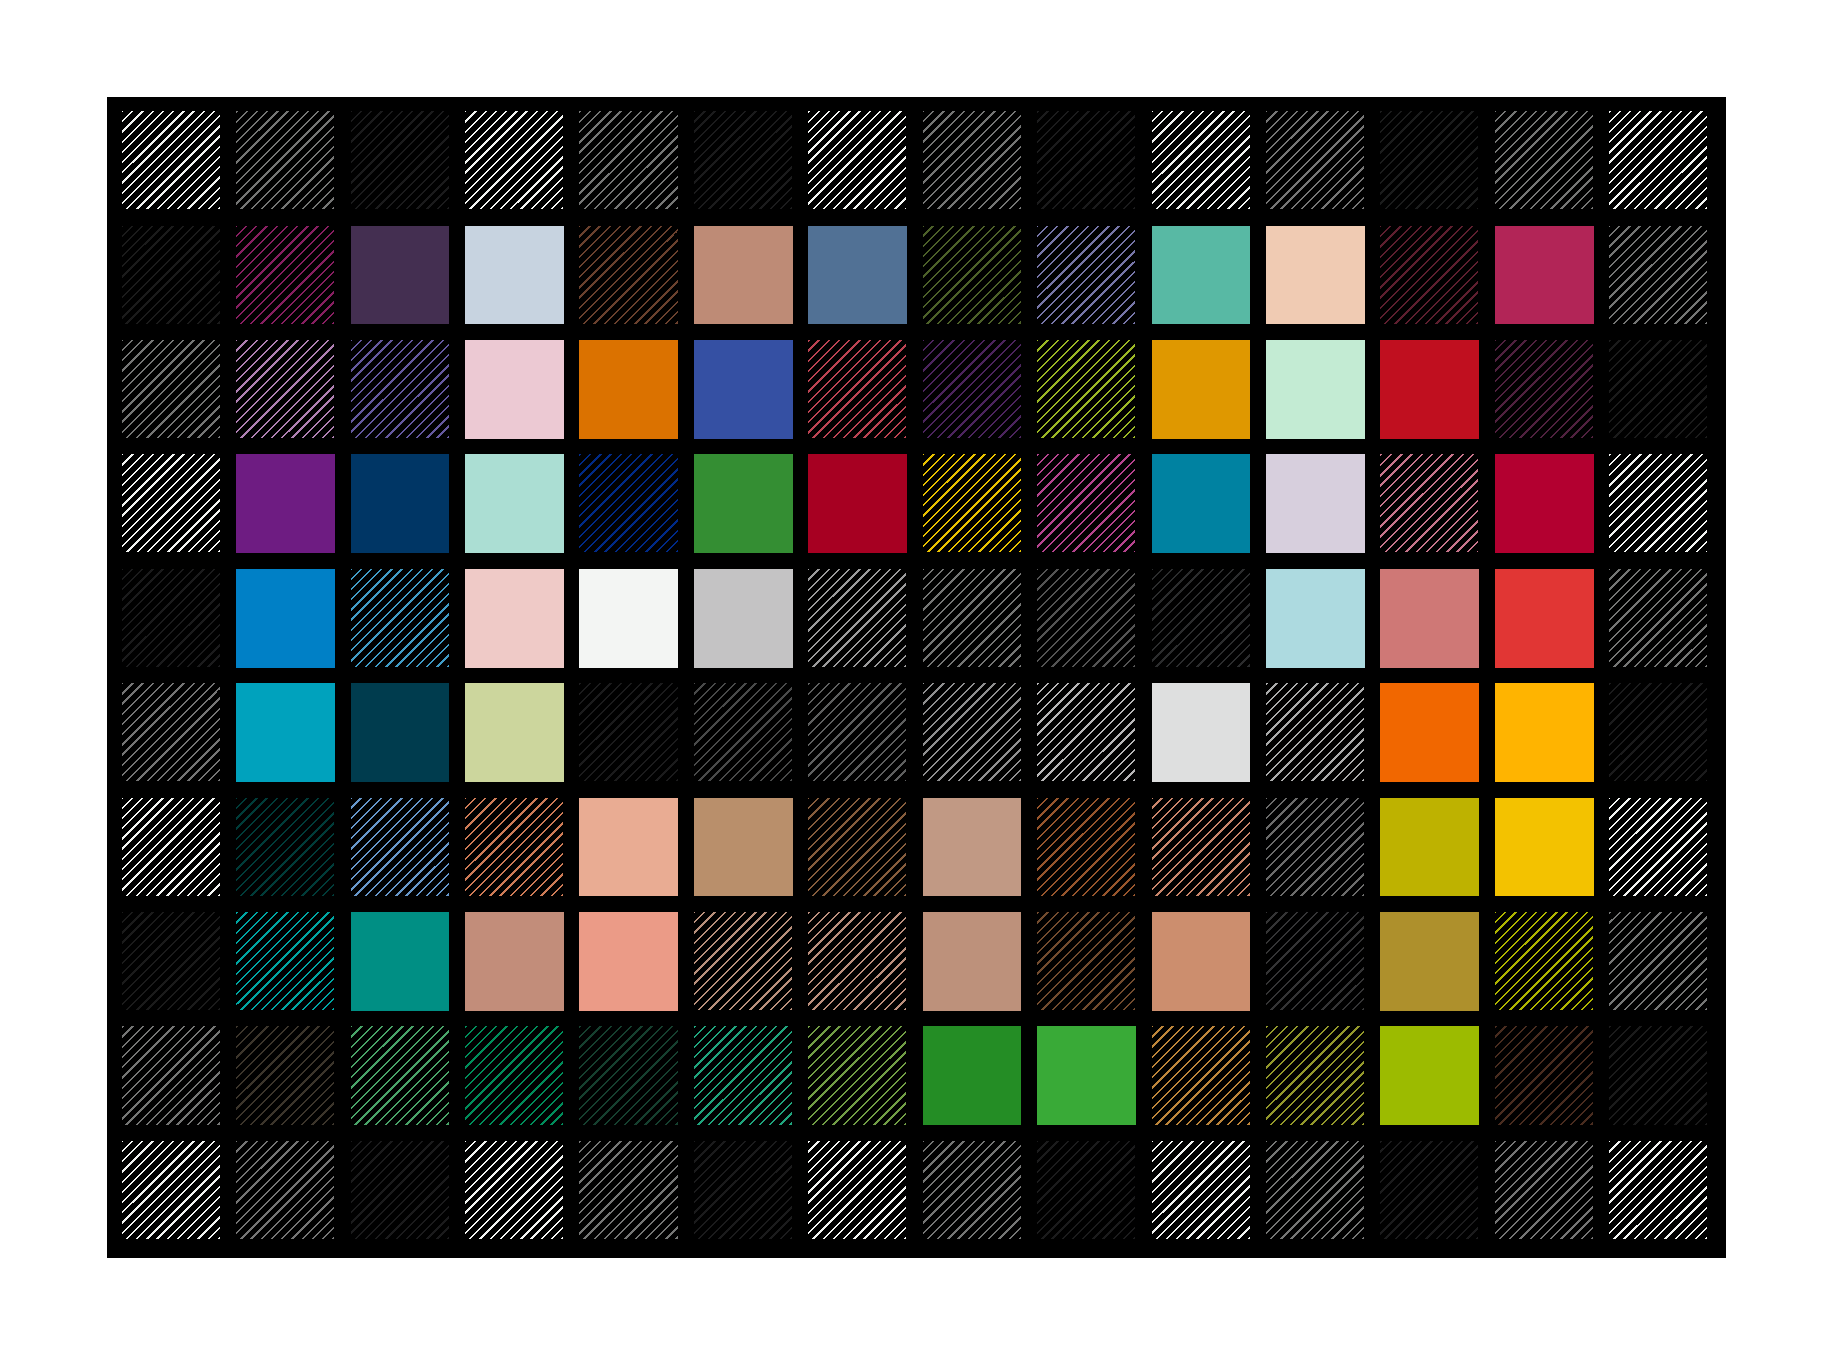
\includegraphics[width=\linewidth]{Fig9a}\\
		(a)
	\end{minipage}%
	\begin{minipage}[b]{0.5\linewidth}
		\centering
		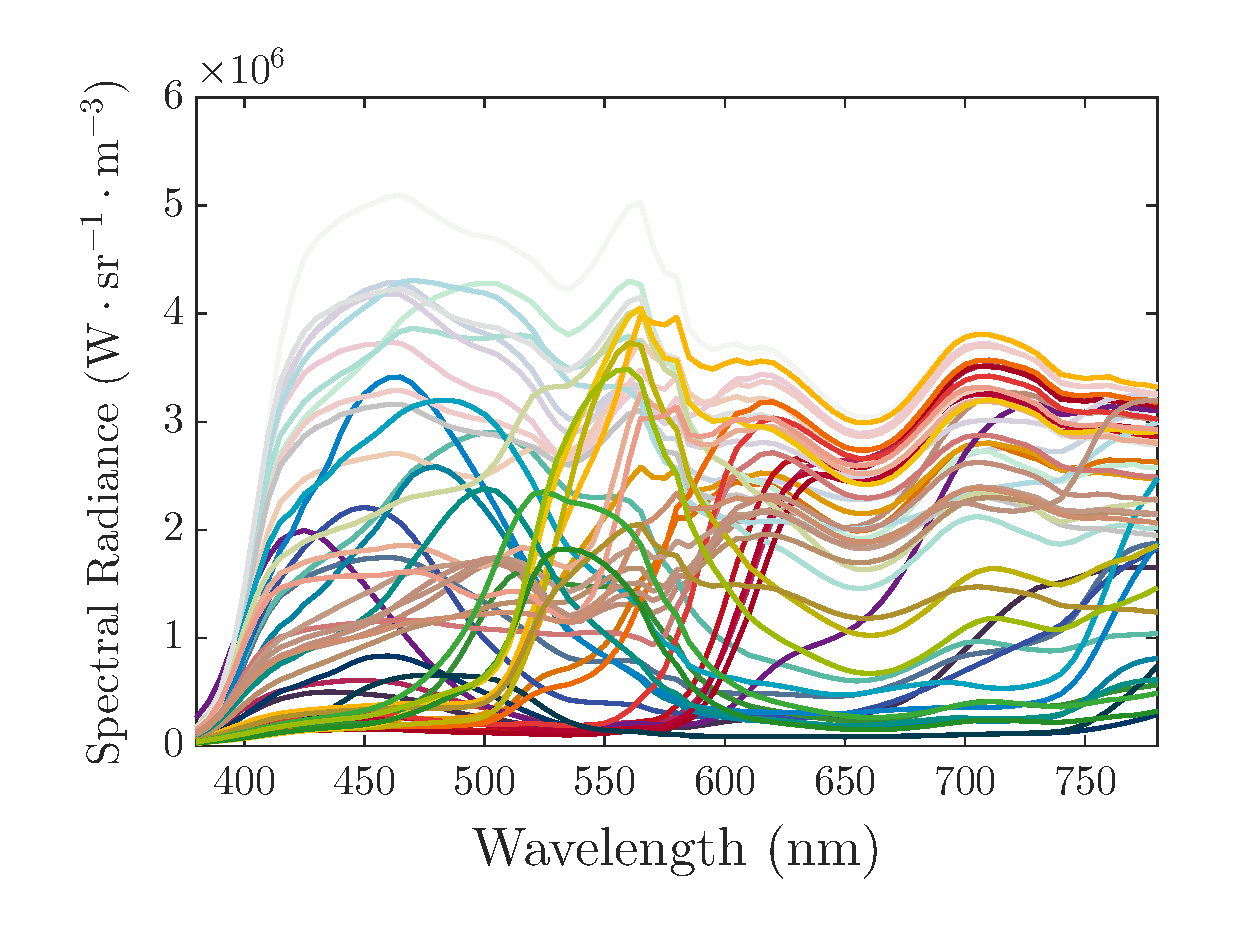
\includegraphics[width=\linewidth]{Fig9b}\\
		(b)
	\end{minipage}
	\caption{(a) The training (plain patches) and testing (hatched patches) samples in our experiments. 44 repeated neutral patches around DSG color checker were discarded through the work, (b) The spectral radiances of 48 selected training samples in the experiments.}
	\label{fig:9}
\end{figure}

\section{Results and discussion}\label{sec:results and discussion}

\subsection{Parameters estimation}\label{sec:parameters estimation}

The initial estimated camera spectral sensitivity $\mathbf{S}_0$, calculated according to \eqref{eq:20}, as well as the optimal camera spectral sensitivity $\mathbf{S}$ after iterations, are illustrated in Fig.~\ref{fig:10}(a). It can be clearly seen that the continuity and smoothness of the initial estimated camera spectral sensitivity are inherited by the optimal one, and the shapes of the two sets of curves coincide closely over the whole spectrum except for some wavebands (for instance 420nm for green channel and 550nm for red channel).

The initial fitting and the optimal result of the nonlinearity, i.e., $(\Phi + c_1)^\beta + c_2$, are plotted in Fig.~\ref{fig:10}(b) for $\Phi\in[0, 1]$, in which the dark current level of Nikon D3x or the y-intercept of nonlinearity curve is close to zero since the dark current is previously suppressed in Nikon’s EXPEED processors before the output of raw data, being distinct from the digital signal processors of other manufacturers.

During the optimization, the value of the cost function converged at 1\% after approximately 20 iterations, as demonstrated in Fig.~\ref{fig:10}(c). It is clearly indicated that our response formation model as well as the interior-point method can significantly improve the accuracy of responses prediction, compared with the traditional spectral characterization method (relatively high cost function value before the iterations).

\begin{figure}[tbp]
	\centering
	\begin{minipage}{0.55\linewidth}
		\centering
		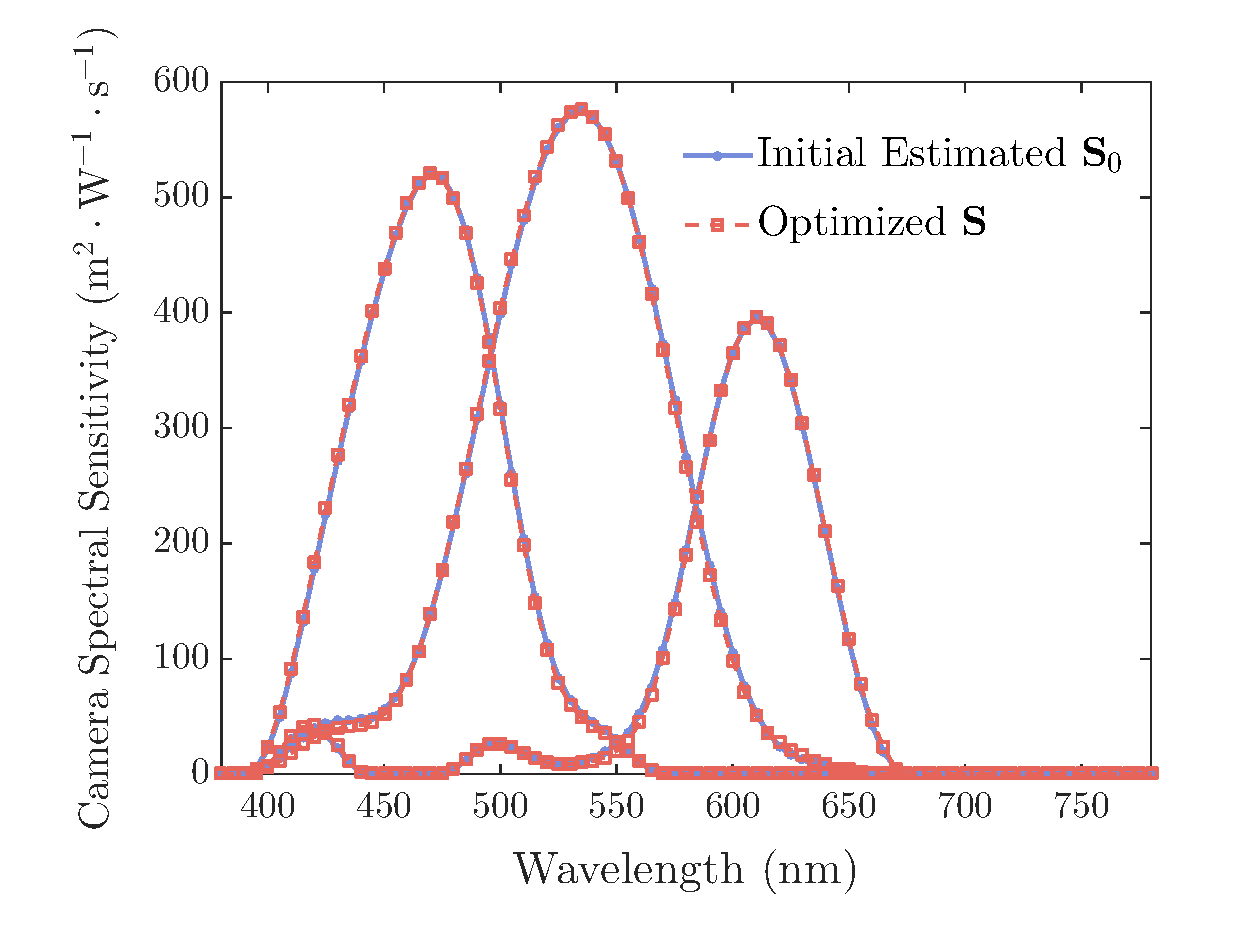
\includegraphics[width=\linewidth]{Fig10a}\\
		(a)
	\end{minipage}\\
	\vspace{0.3em}
	\begin{minipage}[b]{0.5\linewidth}
		\centering
		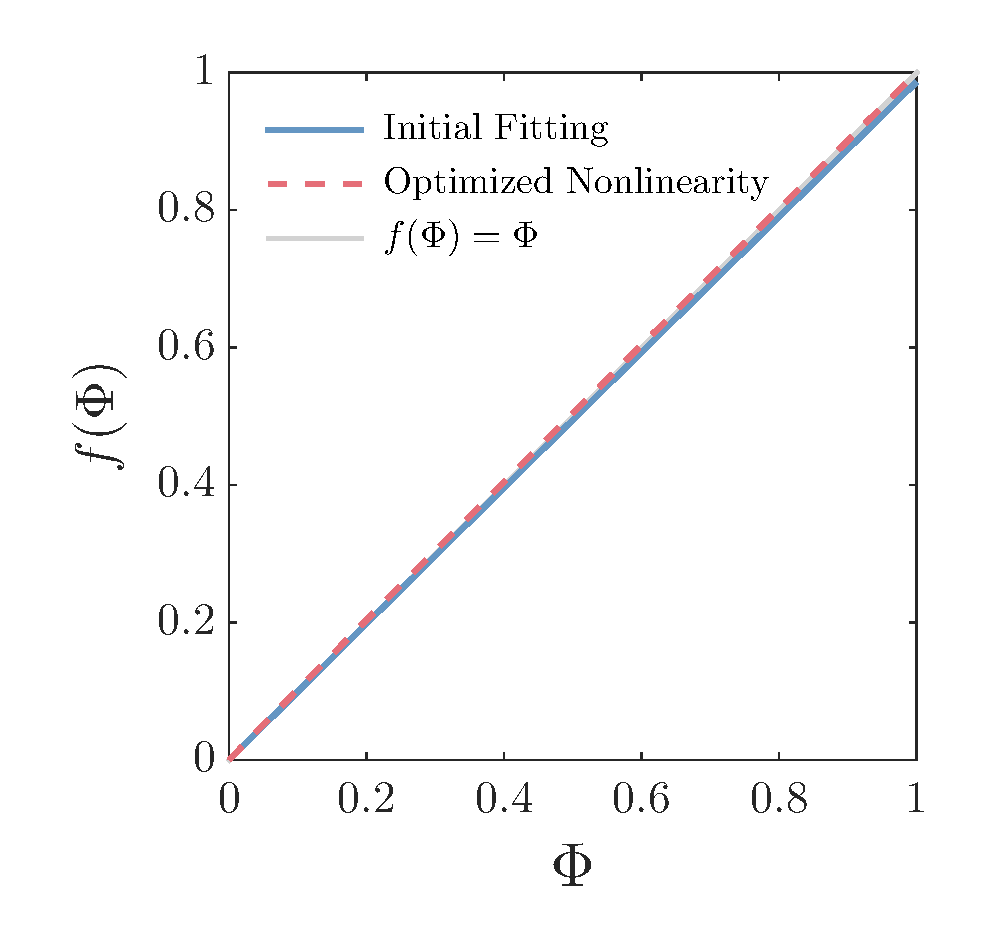
\includegraphics[width=0.85\linewidth]{Fig10b}\\
		(b)
	\end{minipage}%
	\begin{minipage}[b]{0.5\linewidth}
		\centering
		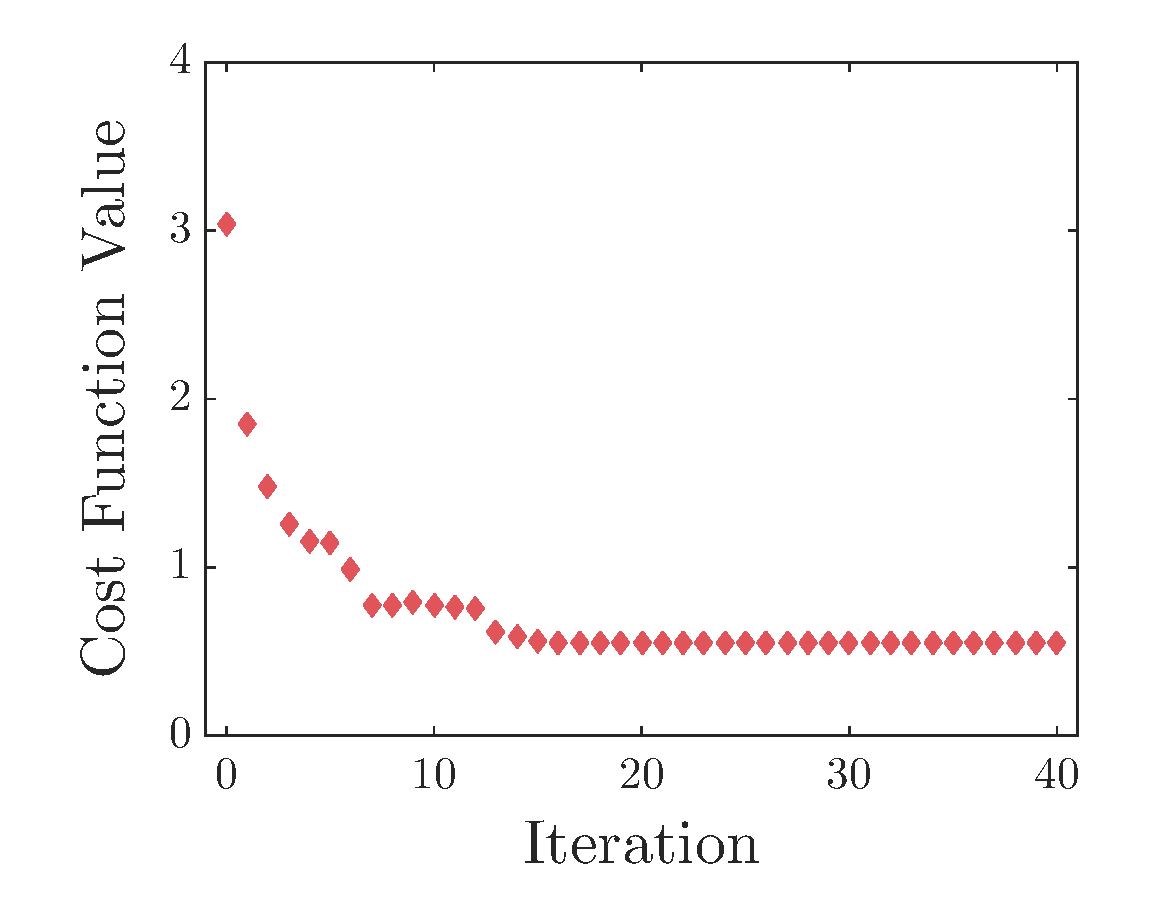
\includegraphics[width=\linewidth]{Fig10c}\\
		(c)
	\end{minipage}
	\caption{(a) The estimated spectral sensitivities of Nikon D3x, (b) The nonlinearity function in the camera response formation model, (c) The value of the cost function during iterations.}
	\label{fig:10}
\end{figure}

Region-dependent parameters, i.e., the crosstalk matrices $\mathbf{C}'$ and the vignetting factors $v$ for the three regions, optimized from \eqref{eq:26}, are listed in Table.~\ref{tab:1}. It clearly demonstrates that the crosstalk effect becomes worse as the target region deviates from the center of the sensor. Since the color filters are located at some distance from the pixel surface due to the metal and insulation layers, the light coming at angles other than orthogonal passes through a filter and can partially be absorbed by the adjacent pixel rather than the one below. The f-number of the lens would also influence the amount of light absorbed by the neighboring pixel~\cite{Agranov:03}, but it is not within the scope here since the relative aperture was fixed. The chromatic aberration of an optical system is another factor that causes the crosstalk, thus the crosstalk matrix in our model is the combination of the pixel spatial crosstalk and the chromatic aberrations.

It should be mentioned that according to the cosine-fourth law, the vignetting factors for the bisected and peripheral regions are approximately 0.81 and 0.49 respectively (the angle of incident light can be calculated given the focal length, sensor’s size and the position of the target region), which are far below the optimized values in Table.~\ref{tab:1}. It is assumed that the difference between the expected and the calculated vignetting factors should result from the elaborate optical design of the lens, which can alleviate the vignetting effect of images, though at the expense of the slight degradation of image quality.

We also compared our estimated camera spectral sensitivity with those obtained by other prevalling methods. Fig.\ref{fig:11} plots five sets of spectral sensitivities estimated by pseudo inverse~\cite{Barnard:02}, radial basis functions network(RBFN)~\cite{Zhao:09}, principal component analysis (PCA)~\cite{Jiang:13}, and our proposed method. The camera spectral sensitivities database to be implemented by PCA and RBFN were downloaded from \url{http://www.cis.rit.edu/~dxl5849/projects/camspec/} and \url{http://www.cvl.iis.u-tokyo.ac.jp/~rei/research/cs/index.html}~\cite{Kawakami:13}, respectively. The notation ``PCA-All'' in Fig.\ref{fig:11} corresponds to the result obtained by performing PCA to all 40 cameras, and ``PCA-Nikon'' to only 12 Nikon cameras. The pseudo inverse method used here is similar to that described in section~\ref{sec:operational details} but only with the regularization constraint.

\begin{figure*}[tbp]
	\centering
	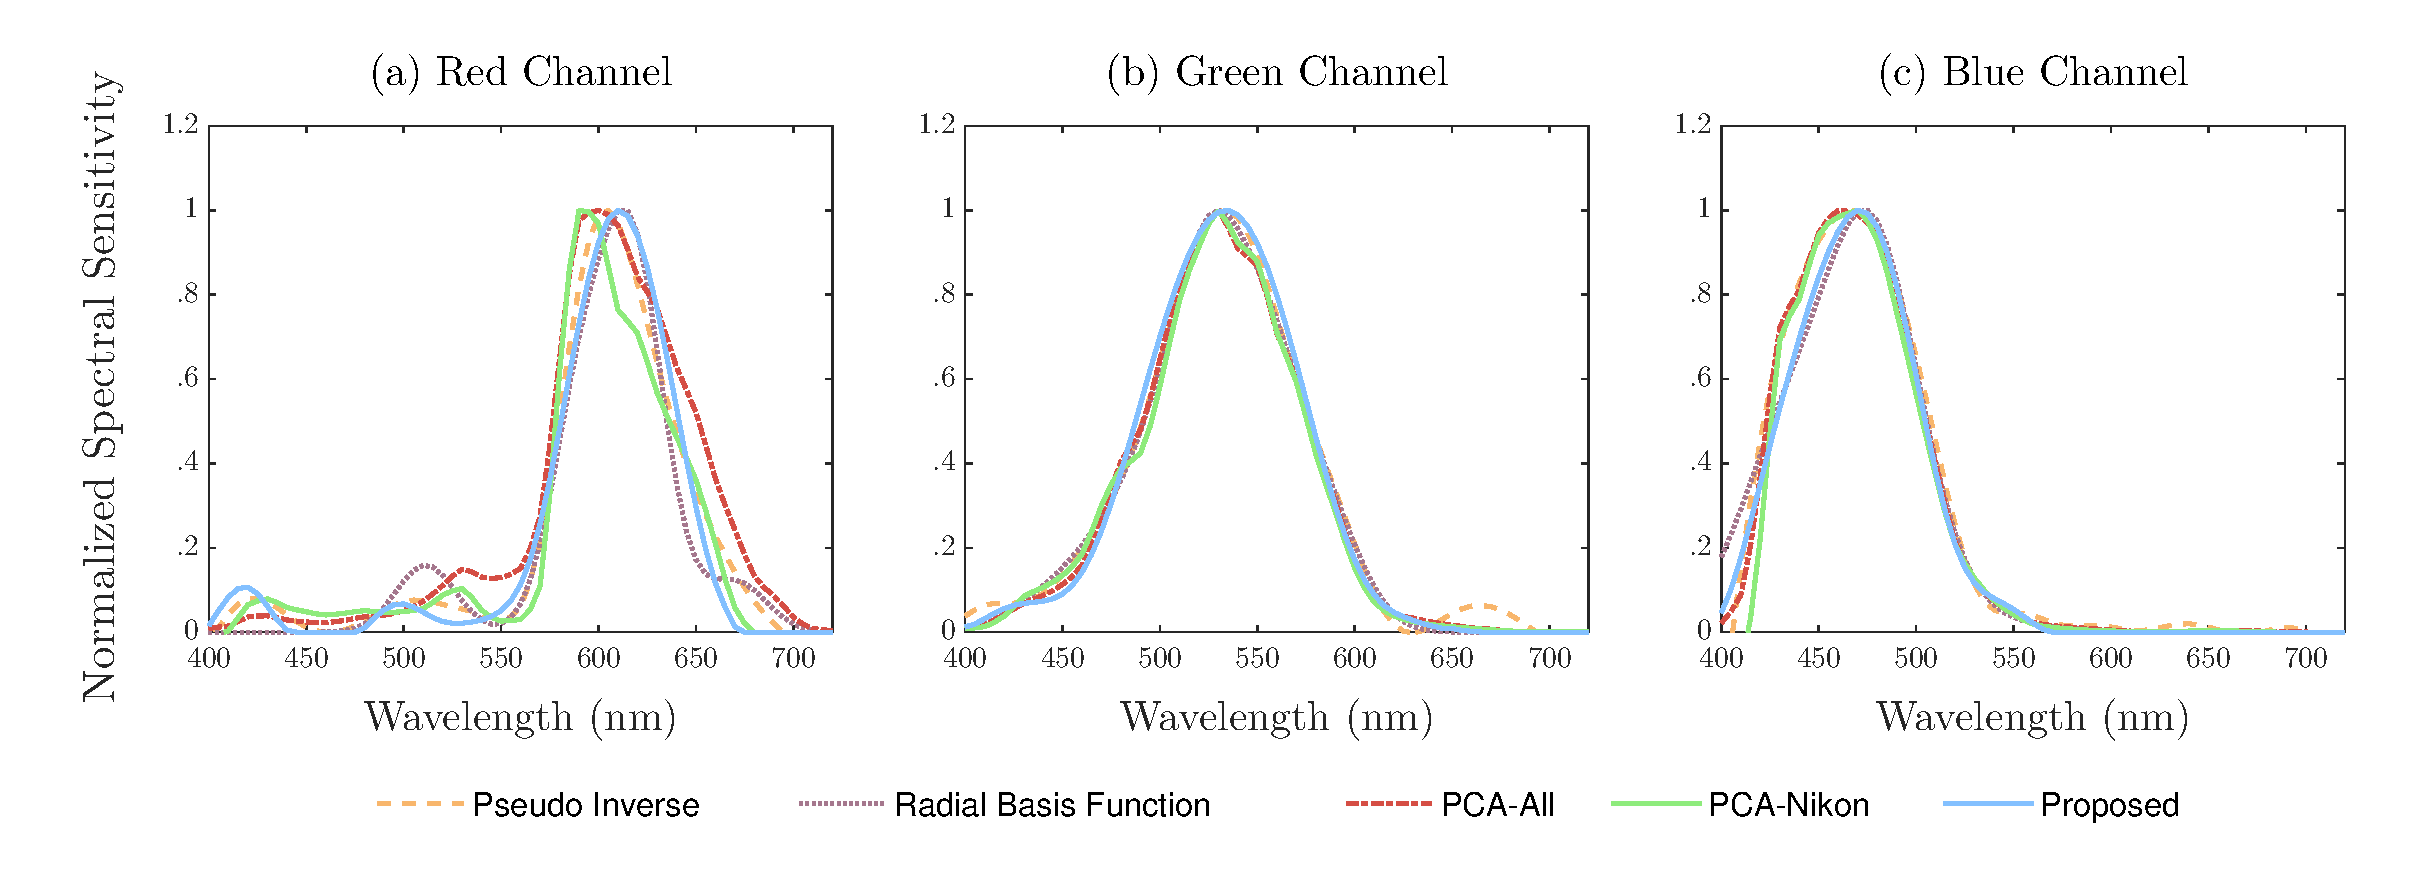
\includegraphics[width=.75\linewidth]{Fig11}
	\caption{Nikon D3x's normalized spectral sensitivities estimated by different methods.}
	\label{fig:11}
\end{figure*}

\begin{table*}[tbph]
	\centering
	\caption{\bf The crosstalk matrices and the vignetting factors for different regions of the sensor}
	{\renewcommand{\arraystretch}{1.6}
		\begin{tabular}{cccc}
			\toprule
			& Central Region & Bisected Region & Peripheral Region \\
			\midrule
			Crosstalk Matrix &%
			$\begin{bmatrix}
			0.9679 & 0.0096 & 0 \\
			0.0027 & 0.9635 & 0.0013 \\
			0	   & 0.0146 & 0.9813 \\
			\end{bmatrix}$ &%
			$\begin{bmatrix}
			0.9592 & 0.0134 & 0 \\
			0.0129 & 0.9649 & 0.0082 \\
			0	   & 0.0305 & 0.9934 \\
			\end{bmatrix}$ &%
			$\begin{bmatrix}
			0.9139 & 0.0607 & 0 \\
			0.0533 & 0.9586 & 0.0576 \\
			0	   & 0.0855 & 0.9825 \\
			\end{bmatrix}$ \\
			Vignetting Factor & $1$ & $0.9496$ & $0.7639$ \\
			\bottomrule
		\end{tabular}}
		\label{tab:1}
	\end{table*}
	
	\subsection{Response prediction}\label{sec:response prediction}
	
	The $\Delta{}E_{00}$ color differences of 48 training samples for different capture settings, obtained by five methods, are shown in Fig.~\ref{fig:12}(a). The error bars represent the 95\% confidence interval of 48 samples under one capture setting (similarly hereinafter). Since the spectral sensitivities estimated by other methods are relative data, they are normalized so that the peak value of each channel is equal to our result, as demonstrated in Fig.~\ref{fig:11}. Thanks to the introduction of crosstalk matrix and the nonlinear parameters, our model show a significant superiority of color prediction over others, especially when the capture setting varies. The prediction accuracy of the traditional methods, without considering the nonequivalence between the exposure time and ISO, goes down when the capture settings are different from the one under which they were calculated, yet the proposed model keeps at the same level.
	
	It should be noted that since the errors caused by the colorimetric characterization applied equally to the actual responses $\mathbf{p}$ and the predicted responses $\hat{\mathbf{p}}$, the color difference between $\mathbf{M}\boldsymbol{\rho}$ and $\mathbf{M}\hat{\boldsymbol{\rho}}$ could be even smaller than those between $\mathbf{M}\boldsymbol{\rho}$ and $\mathbf{p}$.
	
	The distribution of 48 training samples in a*b* plane of CIELAB space are displayed in Fig.~\ref{fig:12}(b), along with the mean color differences for the corresponding samples, in which the radii of circles denote five times of the color difference $\Delta{}E_{00}$ of our model averaged over the data from 5 capture settings (similarly hereinafter).
	
	\begin{figure}[tbp]
		\centering
		\begin{minipage}[b]{0.57\linewidth}
			\centering
			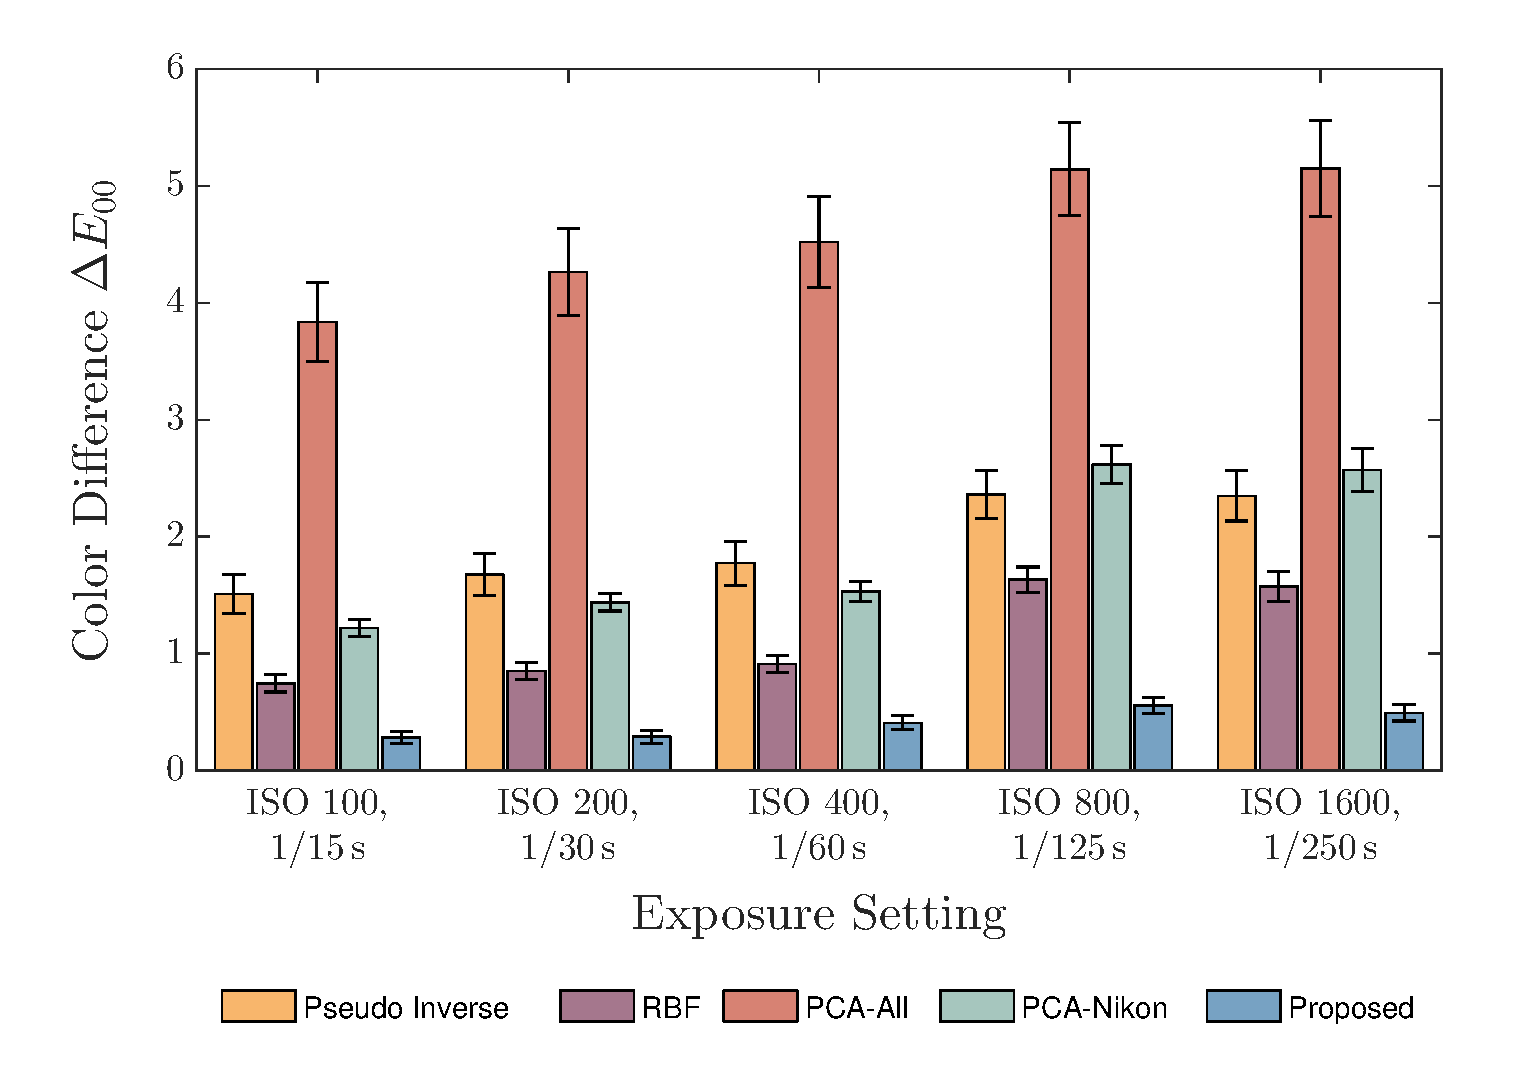
\includegraphics[width=\linewidth]{Fig12a}\\
			(a)
		\end{minipage}%
		\begin{minipage}[b]{0.43\linewidth}
			\centering
			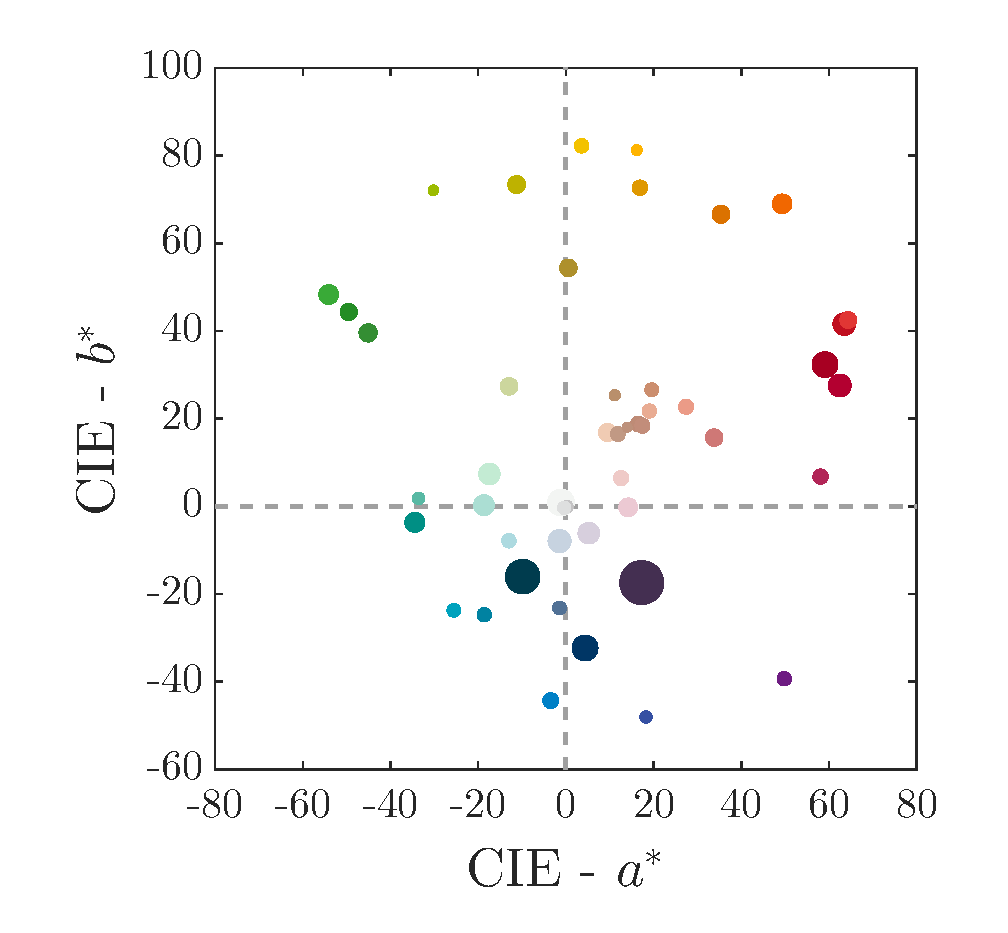
\includegraphics[width=\linewidth]{Fig12b}\\
			(b)
		\end{minipage}
		\caption{(a) Mean CIEDE2000 color difference over 48 training sample under different capture settings, (b) The distribution of training samples in CIELAB $\text{a}^*\text{b}^*$ plane, the radius of circle denotes five times of the mean color difference over five capture settings of our model.}
		\label{fig:12}
	\end{figure}
	
	In the testing phase, we compare the performance of our model with the others for another 48 color samples in ColorChecker DSG, which were excluded from the training phase. The color difference $\Delta{}E_{00}$ for 48 testing samples under different capture settings are shown in Fig.~\ref{fig:13}(a), and Fig.~\ref{fig:13}(b) plots the distribution and the mean color differences of our model of 48 testing samples in CIELAB $\text{a}^*\text{b}^*$ plane. The testing results indicate the perceptively accurate prediction of camera response by our model ($\text{mean}\{\Delta{}E_{00}\} < 0.6$), as well as the tolerance for the worst case ($\text{max}\{\Delta{}E_{00}\} < 2$). The consistency of the prediction accuracies among different capture settings, which is even better than the training results, implies again that our model could be adaptive for various imaging environments, which might require different combinations of capture parameters for obtaining an appropriately exposed image. 
	
	\begin{figure}[tbp]
		\centering
		\begin{minipage}[b]{0.57\linewidth}
			\centering
			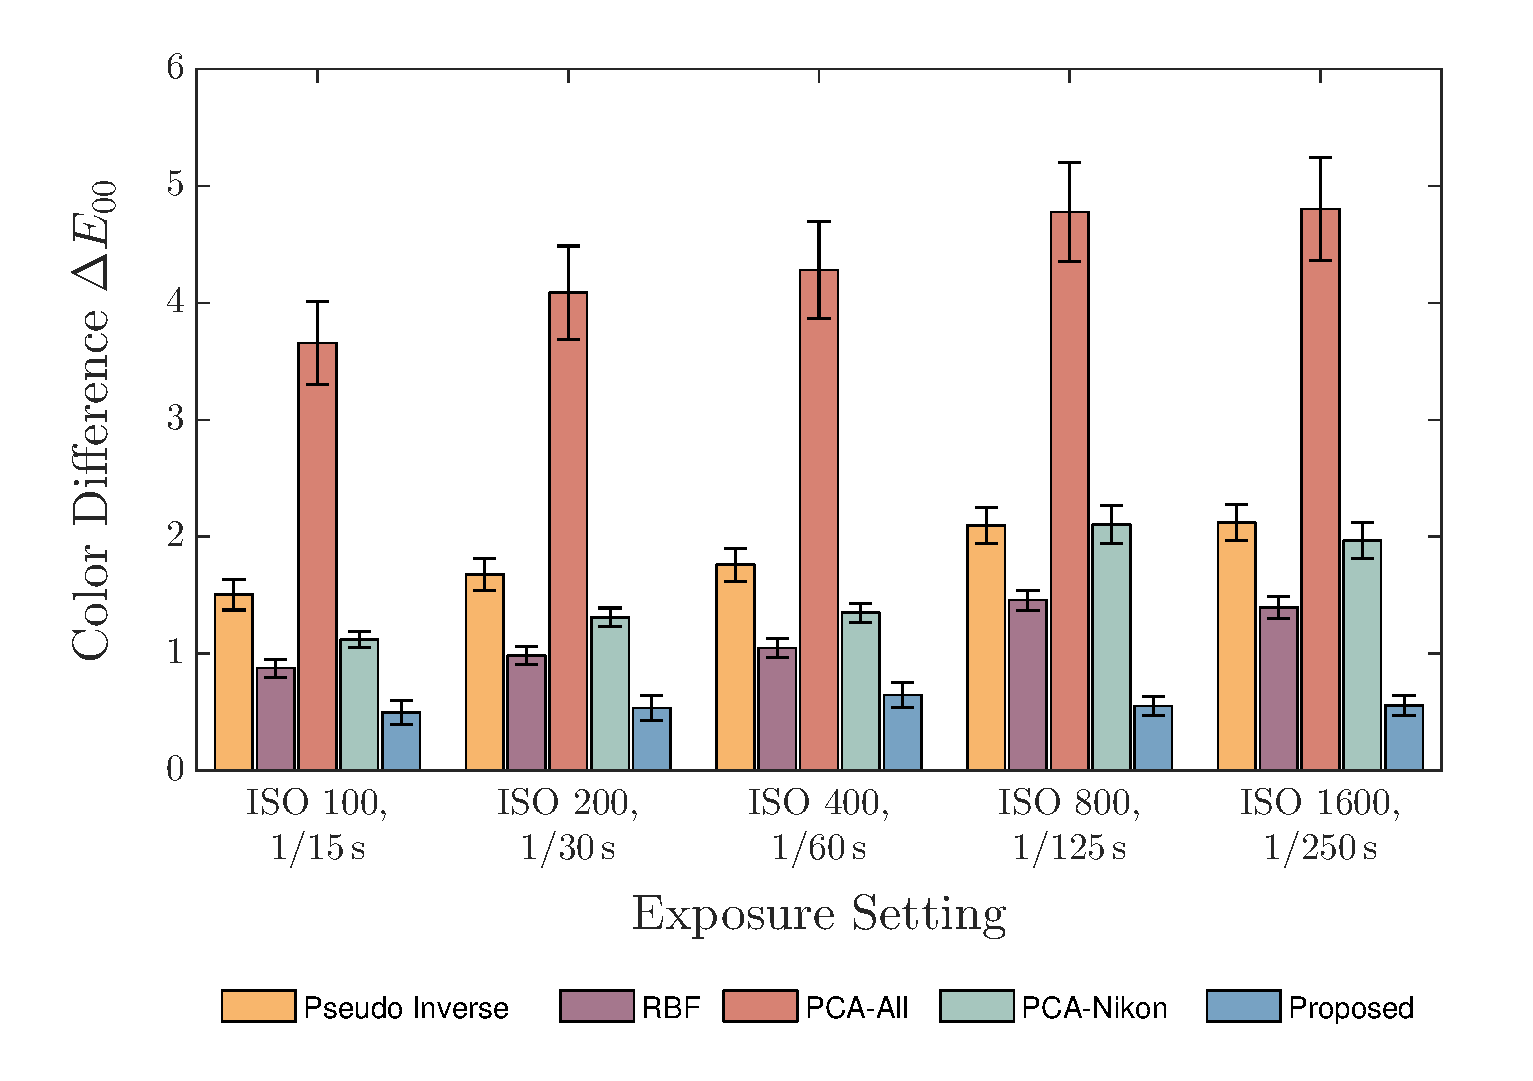
\includegraphics[width=\linewidth]{Fig13a}\\
			(a)
		\end{minipage}%
		\begin{minipage}[b]{0.43\linewidth}
			\centering
			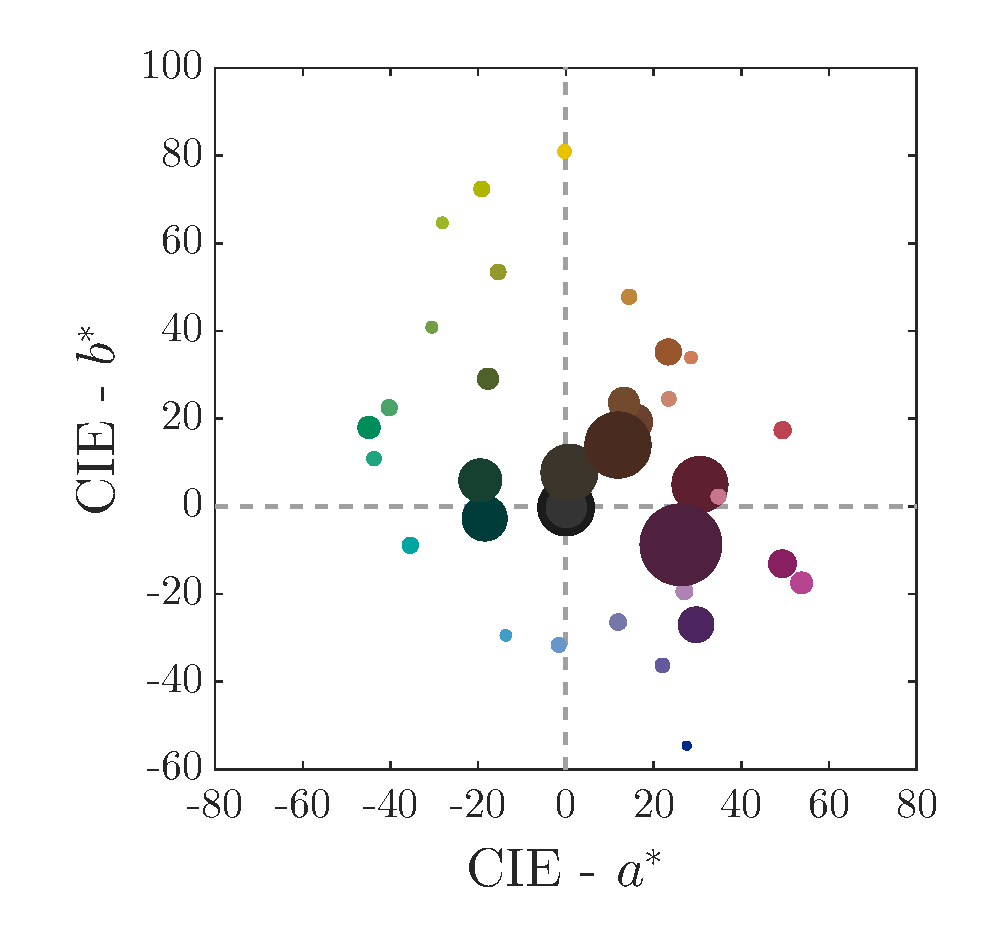
\includegraphics[width=\linewidth]{Fig13b}\\
			(b)
		\end{minipage}
		\caption{(a) Mean CIEDE2000 color difference over 48 testing sample under different capture settings, (b) The distribution of testing samples in CIELAB $\text{a}^*\text{b}^*$ plane.}
		\label{fig:13}
	\end{figure}
	
	Considering the fact that the training and testing samples in the previous experiments might be of high correlation, due to their being illuminated by the same illuminant, the second testing phase was performed, using 24 samples from X-Rite ColorChecker Classic illuminated by A illuminant. To investigate the generalization of our model, the responses of color samples at this testing phase were obtained using the different combinations of exposure time and ISO sensitivity, which did not occur in the training phase. Fig.~\ref{fig:14}(a) plot the color difference $\Delta{}E_{00}$ of 24 color samples captured under settings of (1/20\,s, ISO 125), (1/40\,s, ISO 250), (1/80\,s, ISO 500), (1/160\,s, ISO 1000) and (1/500\,s, ISO 3200), respectively, and the distribution of 24 testing samples in CIELAB $\text{a}^*\text{b}^*$ plane and their corresponding color differences of our model are shown in Fig.~\ref{fig:14}(b).
	
	\begin{figure}[tbp]
		\centering
		\begin{minipage}[b]{0.57\linewidth}
			\centering
			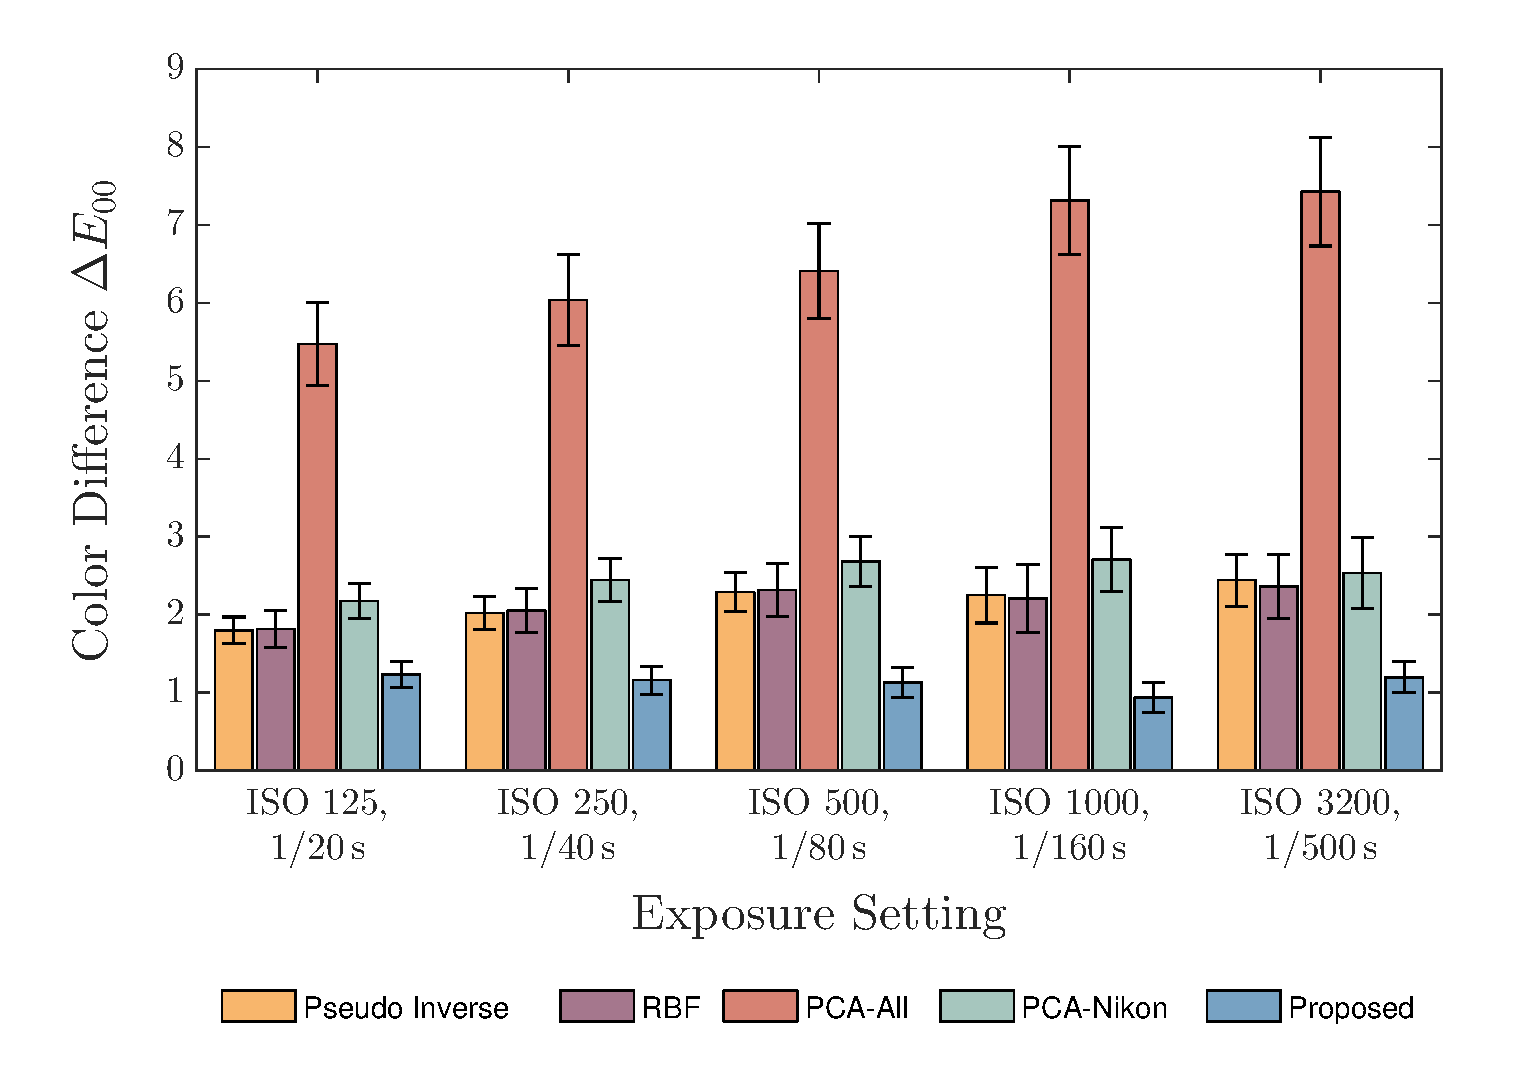
\includegraphics[width=\linewidth]{Fig14a}\\
			(a)
		\end{minipage}%
		\begin{minipage}[b]{0.43\linewidth}
			\centering
			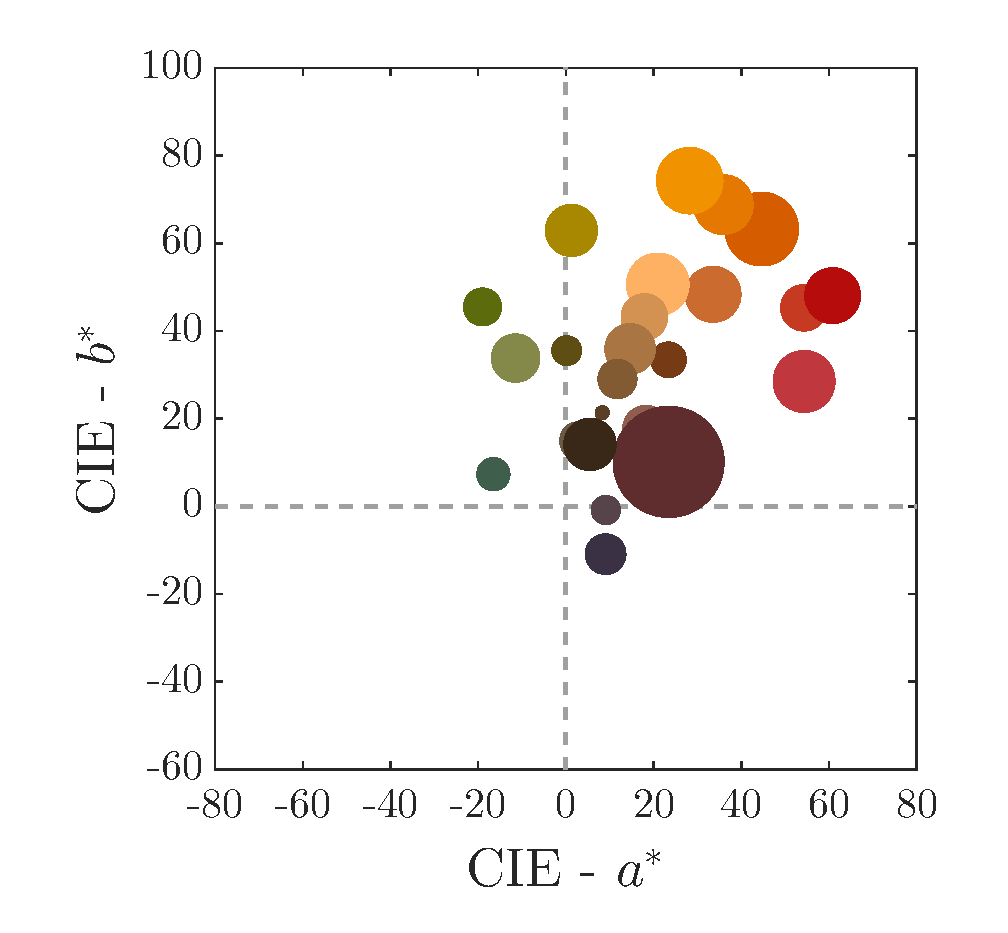
\includegraphics[width=\linewidth]{Fig14b}\\
			(b)
		\end{minipage}
		\caption{(a) Mean CIEDE2000 color difference over 24 testing sample on X-rite ColorChecker Classic, illuminated by illuminant A, under different capture settings, (b) The distribution of testing samples in CIELAB $\text{a}^*\text{b}^*$ plane.}
		\label{fig:14}
	\end{figure}
	
	It is worth noting that by our model, the averaged $\Delta{}E_{00}$ of the responses under the setting of (1/500\,s, ISO 3200) is still at a competitive level ($\Delta{}E_{00}\approx1$), even though both the exposure time and the ISO sensitivity value exceed the extreme of the training phase.
	
	\section{Conclusion}\label{conclusion}
	
	In this study, a camera response formation model was developed to accurately predict the camera responses using the optimized camera spectral sensitivity and the nonlinearity function. The testing phase indicates that our model can achieve high-fidelity color reproduction for images captured under various camera settings. The prediction results of testing samples, whose spectral radiances and capture settings distinctly differ from the training ones, verifies the generalization ability of our model. The experiments support the hypothesis that the crosstalk effect is a non-negligible factor in camera response formation, and a $3\times3$ crosstalk matrix can reasonably explain the difference of responses over different regions of the sensor. If enough regions on sensors were to be investigated, a complete imaging simulator would be created. Since the image responses under different environments can be simulatively obtained, the colorimetric and photometric research and applications based on the cameras would be much of convenience and efficiency.
	
	\section*{Acknowledgments}\label{acknowledgments}
	This work was supported by the National Basic Research Program of China under Grant No. xxxxxxxxxx.
	
	\bigskip
	
	% Bibliography
	\bibliography{Bibliography_revised.bib}
\end{document}